\documentclass[10pt,oneside]{article}

\usepackage{xcolor}
\usepackage{cancel}
\usepackage{bm}
\usepackage{graphicx}
\usepackage{hyperref}
\usepackage{adjustbox}
\hypersetup{colorlinks, allcolors=.,urlcolor=structure}
\usepackage{booktabs}  % for top and bottom spacing in table cells, \addlinespace
\usepackage[x11names, svgnames]{xcolor} % for colors in handouts, auto loaded in Beamer?
\usepackage{tikz}
\usetikzlibrary{arrows.meta, math, calc, shadows,bending}
\usetikzlibrary{decorations.markings, decorations.fractals, decorations.text} % for chain, etc.
\usetikzlibrary{intersections}
\usepackage{pgfmath}
\usepackage{ifthen}
\usepgfmodule{oo}
\usetikzlibrary{shadings}
% \usetikzlibrary{decorations.shapes}
\usepackage[many]{tcolorbox}
\tcbuselibrary{skins} % for image boxes
\usepackage[absolute,overlay,showboxes]{textpos}
% \usepackage{textpos}
% \textblockorigin{0.0cm}{0.0cm}  %start all at upper left corner
\TPshowboxesfalse

\newcommand\lb{\linebreak}
\newcommand\Ra{\Rightarrow}
\newcommand\cd{\!\cdot\!}
\newcommand\x{\!\times\!}
\newcommand\pars{\par\smallskip}
\newcommand\parm{\par\medskip}
\newcommand\parb{\par\bigskip}
\renewcommand{\deg}{^\circ}

% counter for resuming enumerated list numbers
\newcounter{resumeenumi}
\newcommand{\suspend}{\setcounter{resumeenumi}{\theenumi}}
\newcommand{\resume}{\setcounter{enumi}{\theresumeenumi}}



% https://tex.stackexchange.com/questions/33703/extract-x-y-coordinate-of-an-arbitrary-point-in-tikz
\makeatletter
\providecommand{\gettikzxy}[3]{%
	\tikz@scan@one@point\pgfutil@firstofone#1\relax
	\edef#2{\the\pgf@x}%
	\edef#3{\the\pgf@y}%
}
\makeatother

\makeatletter
\newcommand{\verbatimfont}[1]{\def\verbatim@font{#1}}%
\makeatother

%%%%%%%%%%%%%%%%%%%%%%%%%%%%%%%%%%%%%%%%%%%%%%%%%%%%%%%%%%%%%%%%%%%%%%%%%%%%%%%%


% \newcommand{\tb}[4][0.8]{
% 	\begin{textblock*}{#1}(#2, #3)
% 		\raggedright
% 		#4
% 	\end{textblock*}
% }

% \def\tb

\newtcolorbox{statsbox}[2][] { 
  colback=white,
  colbacktitle=structure,
  colframe=structure,
  coltitle=white,  
  top=0.25cm,
	bottom=0.125cm,
	left=0mm,
	right=0mm,
  % fonttitle=\itshape\rmfamily,
  halign=flush left, 
  enhanced,
  drop fuzzy shadow,
  attach boxed title to top left={xshift=3.5mm, yshift=-2mm},
  title={#2}, #1}
\newtcolorbox{redbox}{colback=white, colframe=structure, enhanced, drop fuzzy shadow}
\newtcolorbox{titledbox}[1]{colback=white,colframe=structure,title={#1}}
\newtcbox{\tcb}[1][]{colback=white,boxsep=0pt,top=0.5cm,bottom=0.5cm,left=0.5cm,
		right=0.5cm, colframe=structure,  enhanced, drop fuzzy shadow, #1}
\newtcbox{\tcbfig}[1][1]{colback=white,boxsep=0pt,top=0.5cm,bottom=0.5cm,left=0.5cm,
		right=0.5cm, colframe=structure,  enhanced, drop fuzzy shadow, #1}
% tcb title
\newtcbox{\tcbt}[2][]{colback=white,boxsep=0pt,top=5pt,bottom=5pt,left=5pt,
		right=5pt, colframe=structure, enhanced, drop fuzzy shadow,  title={#2}, #1}
% tcb left title
\newtcbox{\tcbtl}[2][]{ colback=white,
  colbacktitle=structure,
  colframe=structure,
  coltitle=white,  
  top=0.25cm,
	bottom=0.125cm,
	left=0mm,
	right=0mm,
  % fonttitle=\bfseries,
  halign=flush left, 
  enhanced,
  drop fuzzy shadow,
  attach boxed title to top left={xshift=3.5mm, yshift=-2mm}, 
	title={#2}, #1}

\newtcbtheorem{myexam}{Example}%
{
	enhanced,
	colback=white,
	colframe=structure,
	% fonttitle=\bfseries,
	fonttitle=\itshape\rmfamily,
	drop fuzzy shadow,
	%description font=\mdseries\itshape,
	attach boxed title to top left={yshift=-2mm, xshift=5mm},
	colbacktitle=structure
	}{exam}% then \pageref{exer:theoexample} references the theo

% \newcommand{\myexample}[2][red]{
% 	% \tcb\tcbset{theostyle/.style={colframe=red,colbacktitle=yellow}}
% 	\begin{myexam}{}{}
% 		#2
% 	\end{myexam}
% 	% \tcbset{colframe=structure,colbacktitle=structure}
% }

\newtcbtheorem{myexer}{Exercise}%
{
	enhanced,
	colback=white,
	colframe=structure,
	% fonttitle=\bfseries,
	drop fuzzy shadow,
	fonttitle=\itshape\rmfamily,
	% description font=\mdseries\itshape,
	attach boxed title to top left={yshift=-2mm, xshift=5mm},
	colbacktitle=structure
	}{exer}



\newcommand{\mini}[2][0.8]{
	\begin{minipage}[c]{#1\columnwidth}
		\raggedright
		#2
	\end{minipage}
}
\newcommand{\minit}[2][0.8]{
	\begin{minipage}[t]{#1\columnwidth}
		% \raggedright
		#2
	\end{minipage}
}

% centered minipage with text \raggedright
%\cmini[width]{content}
\newcommand{\cmini}[2][0.8]{
	\begin{center}
		\begin{minipage}{#1\columnwidth}
			\raggedright
			#2
		\end{minipage}
	\end{center}
}

\newcommand{\fig}[2][1]{% scaled graphic
	\includegraphics[scale=#1]{#2}
}

% centred framed box black border
%\cbox[width]{content}
\newcommand{\cbox}[2][1]{% framed centered color box
	\setlength\fboxsep{5mm}
	\setlength\fboxrule{.2 mm}
	\begin{center}
		\fcolorbox{black}{white}{
			\vspace{-0.5cm}
			\begin{minipage}{#1\columnwidth}
				\raggedright
				#2
			\end{minipage}
		}
	\end{center}
	\setlength\fboxsep{0cm}
}

\newcommand{\ccbox}[4][1]{% framed centered color box
	\setlength\fboxsep{5mm}
	\setlength\fboxrule{.2 mm}
	\begin{center}
		\fcolorbox{#2}{#3}{
			% \vspace{-0.5cm}
			\begin{minipage}{#1\columnwidth}
				\vspace{-0.25cm}
				\raggedright				
				#4
				\vspace{-0.325cm}
			\end{minipage}
		}
	\end{center}
	\setlength\fboxsep{0cm}
}

\newcommand{\cfig}[2][1]{% centred, scaled graphic
	\begin{center}
		% \fcolorbox{structure}{white}{
		\tcbincludegraphics{
			\includegraphics[scale=#1]{#2}
		}
	\end{center}
}

% figure with tight border for photos
% \cfigb[saitMaroon]{borderwidth with unit}{scale}{image}
\newcommand{\stcsfig}[2][1]{
	% \usepackage{adjustbox}
	% \setlength{\fboxrule}{1pt}
	\begin{center}
		\tcbincludegraphics[width=#1\textwidth, boxrule=2pt, top=-3pt, right=-3pt, left=-3pt, bottom=-3pt,colframe=structure, sharp corners, enhanced, drop fuzzy shadow]{#2}
	\end{center}
}






 \definecolor{saitPurple}{RGB}{112,40,119}
 \definecolor{statsMaroon}{rgb}{0.55, 0, 0}
 \definecolor{saitMaroon}{rgb}{0.55, 0, 0}
 \definecolor{saitRed}{RGB}{224,38,37}
 \definecolor{saitBlue}{rgb}{0, 0.59, 0.85}
 \definecolor{statsDeepBlue}{RGB}{0, 99, 167}
 \definecolor{saitDeepBlue}{RGB}{0, 99, 167}
 \definecolor{LightGrey}{RGB}{200,200,200}
%  \definecolor{boxBG}{RGB}{236, 227, 227}
%  \definecolor{boxBG}{RGB}{242, 233, 223}
%\Member{startpt}{endpt}{outer fill color}{inner fill color}{stroke}{height}{radius}{linewidth}
\providecommand{\Member}[8]{
  % name the points
  \coordinate(start) at (#1);
  \coordinate(end) at (#2);
  \edef\ofill{#3}%
  \edef\ifill{#4}%
  \edef\stroke{#5}%
  \edef\height{#6} % cm
  \edef\radius{#7} % cm
  \edef\linewidth{#8} % mm

  \coordinate(delta) at ($ (end)-(start) $);
  \gettikzxy{(delta)}{\dx}{\dy}
  \gettikzxy{(start)}{\sx}{\sy}
  \pgfmathparse{veclen(\dx, \dy)} \let\length\pgfmathresult

  \pgfmathparse{\dx==0}%
  % \ifnum low-level TeX for integers
  \ifnum\pgfmathresult=1 % \dx == 0
    \pgfmathsetmacro{\rot}{\dy > 0 ? 90 : -90}
  \else
    \pgfmathsetmacro{\rot}{\dx > 0 ? atan(\dy / \dx) : 180 + atan(\dy / \dx)}
  \fi

  
   
  \shadedraw[transform canvas = { rotate around = {\rot:(\sx,\sy)}}, line width = \linewidth, rounded corners = \radius mm, top color = \ofill, bottom color = \ofill, middle color = \ifill, draw = \stroke] ($ (start)+(-0.5*\height, 0.5*\height) $) -- ++(\height cm +\length pt, 0 ) -- ++(0, -\height) -- ++ (-\height cm -\length pt, 0) -- cycle;


  \shadedraw[ball color = \ofill!50!\ifill, draw = \stroke] (start) circle (\height/8);
  \shadedraw[ball color = \ofill!50!\ifill, draw = \stroke] (end) circle (\height/8);
  %  \pgfresetboundingbox

  
  


}


\newcommand{\PC}[6][0]{%
  \edef\lrotate{#1}%
  \edef\lpin{#2}%
  \edef\lfill{#3}%
  \edef\ldraw{#4}%
  \edef\lscale{#5}%
  \edef\lwidth{#6}%
  \edef\h{1}%
  \edef\r{0.3}%
  \begin{scope}[scale=\lscale, rotate=\lrotate]
	\filldraw[draw=\ldraw, fill=\lfill, line width=\lwidth mm] ($ (\lpin) + (0.201*\h+1.0353*\r ,-0.75*\h) $) -- ++(105: 0.77646*\h+0.26795*\r) arc (15:165:\r) -- ++(-105:0.77646*\h+0.26795*\r) -- cycle;

	\shadedraw[ball color=\lfill, draw=\ldraw, line width = \lwidth mm] (\lpin) circle (1.5mm);

	\filldraw[rounded corners=\lscale pt, draw=\ldraw, fill=\lfill, line width=\lwidth mm] ($ (\lpin) - (1,1) $) rectangle +(2,0.25);
  \end{scope}%
}




% \setlength{\TPHorizModule}{1.0cm}
% \setlength{\TPVertModule}{\TPHorizModule}


\usepackage[letterpaper]{geometry}
\geometry{verbose,tmargin=0.25in,bmargin=0.5in,lmargin=1in,rmargin=1.06in}

% https://tex.stackexchange.com/questions/731957/how-to-supress-missing-character-there-is-no-u003b-in-font-nullfont
\tracinglostchars=1

\hfuzz=150pt
\setlength{\parindent}{0pt}

\begin{document}

%%%%%%%%%%%%%%%%%%%%%%%%%%%%%%%%%%%%%%%%%%%%%%%%%%%%%%%%%%%%%%%%%%%%%%%%%%%%%%%%%%%%%%%%%%%%%%%%%%%%
% page 1
%%%%%%%%%%%%%%%%%%%%%%%%%%%%%%%%%%%%%%%%%%%%%%%%%%%%%%%%%%%%%%%%%%%%%%%%%%%%%%%%%%%%%%%%%%%%%%%%%%%%

\begin{textblock*}{7.25in}(1in, 0.4in)
	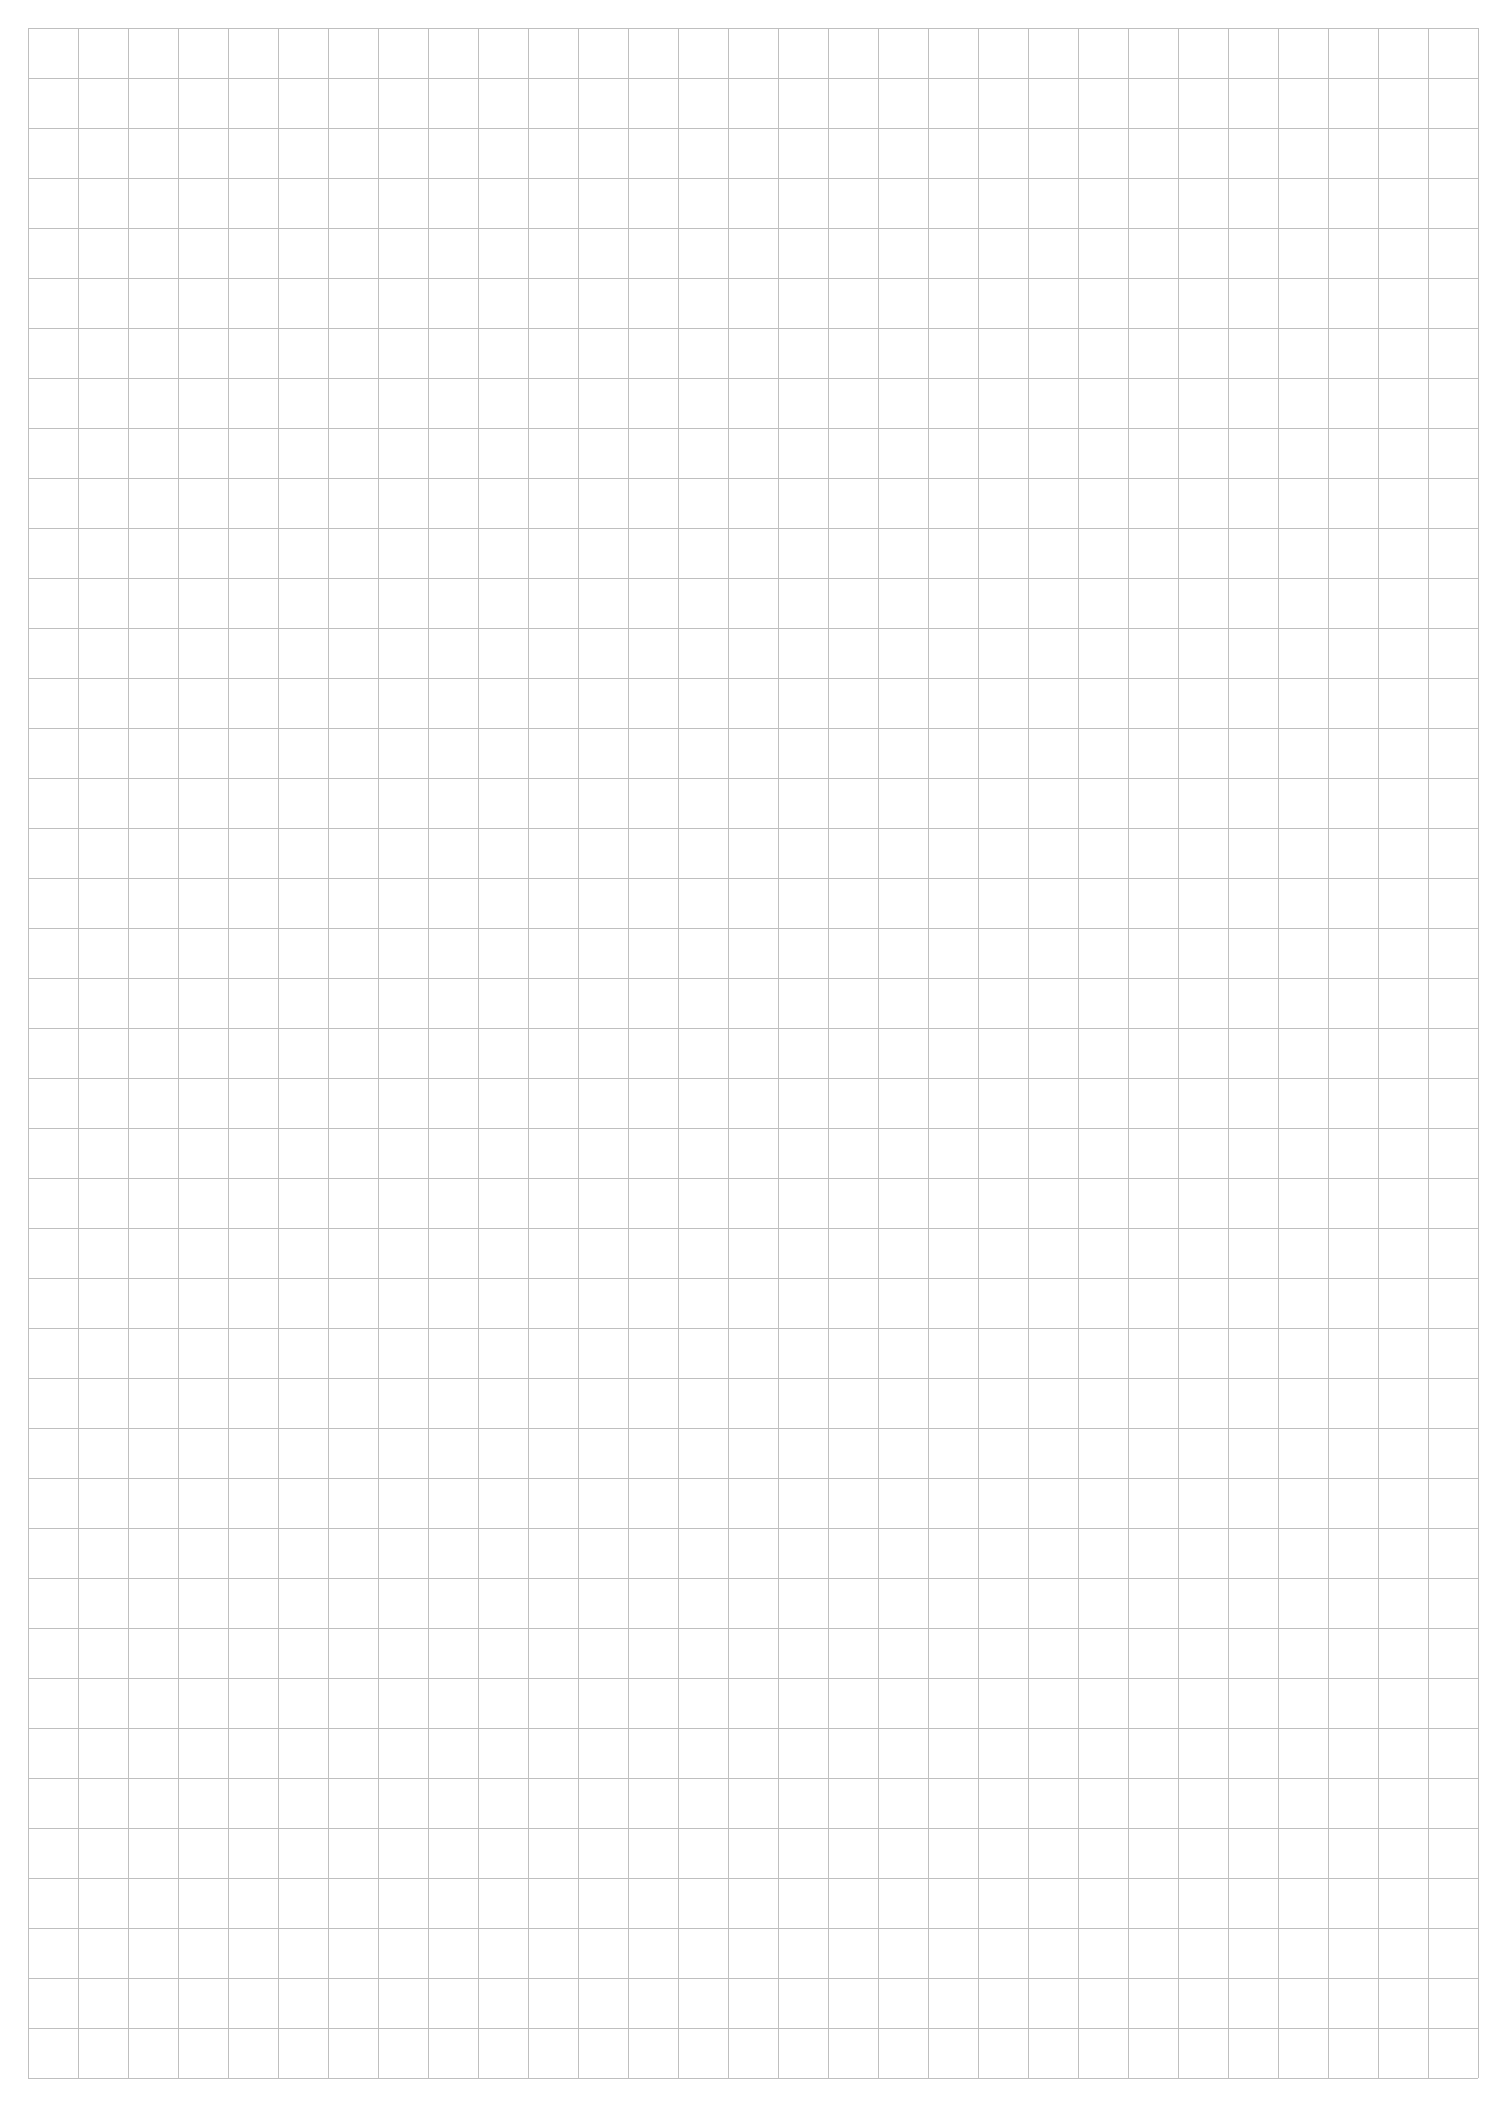
\begin{tikzpicture}[line width=0.1mm]
		\draw[color=gray!50, step=0.25in] (0,0) grid +(7.25in,10.25in);
	\end{tikzpicture}
\end{textblock*}


\begin{textblock*}{6.75in}(1in, 0.225in)
  \cbox{
    \centering\huge
    \textbf{Engineering Statics - 01 Math Review Handout}
  }
\end{textblock*}


\begin{textblock*}{2in}(1in, 1in)
	\cbox{
    \vspace{-0.25cm}
		1) Solve $a^2=b^2+c^2$ for $b$.
    \vspace{-0.5cm}
	}
\end{textblock*}


\begin{textblock*}{2in}(1in, 3in)
	\cbox{
    \vspace{-0.25cm}
		2) Solve $V=\frac43 \pi r^3$ for $r$.
    \vspace{-0.5cm}
	}
\end{textblock*}


\begin{textblock*}{3in}(1in, 5in)
	\cbox{
    \vspace{-0.25cm}
		3) Solve $c^2=a^2+b^2-2bc\cos C$ for $\cos C$.
    \vspace{-0.5cm}
	}
\end{textblock*}


\begin{textblock*}{3in}(1in, 7.75in)
	\cbox{
    \vspace{-0.25cm}
		4) Solve $b^2=a^2+c^2-2ac\cos B$ for $B$.
    \vspace{-0.5cm}
	}
\end{textblock*}

%%%%%%%%%%%%%%%%%%%%%%%%%%%%%%%%%%%%%%%%%%%%%%%%%%%%%%%%%%%%%%%%%%%%%%%%%%%%%%%%%%%%%%%%%%%%%%%%%%%%
% page 2
%%%%%%%%%%%%%%%%%%%%%%%%%%%%%%%%%%%%%%%%%%%%%%%%%%%%%%%%%%%%%%%%%%%%%%%%%%%%%%%%%%%%%%%%%%%%%%%%%%%%

.\newpage

\begin{textblock*}{7.25in}(1in, 0.4in)
	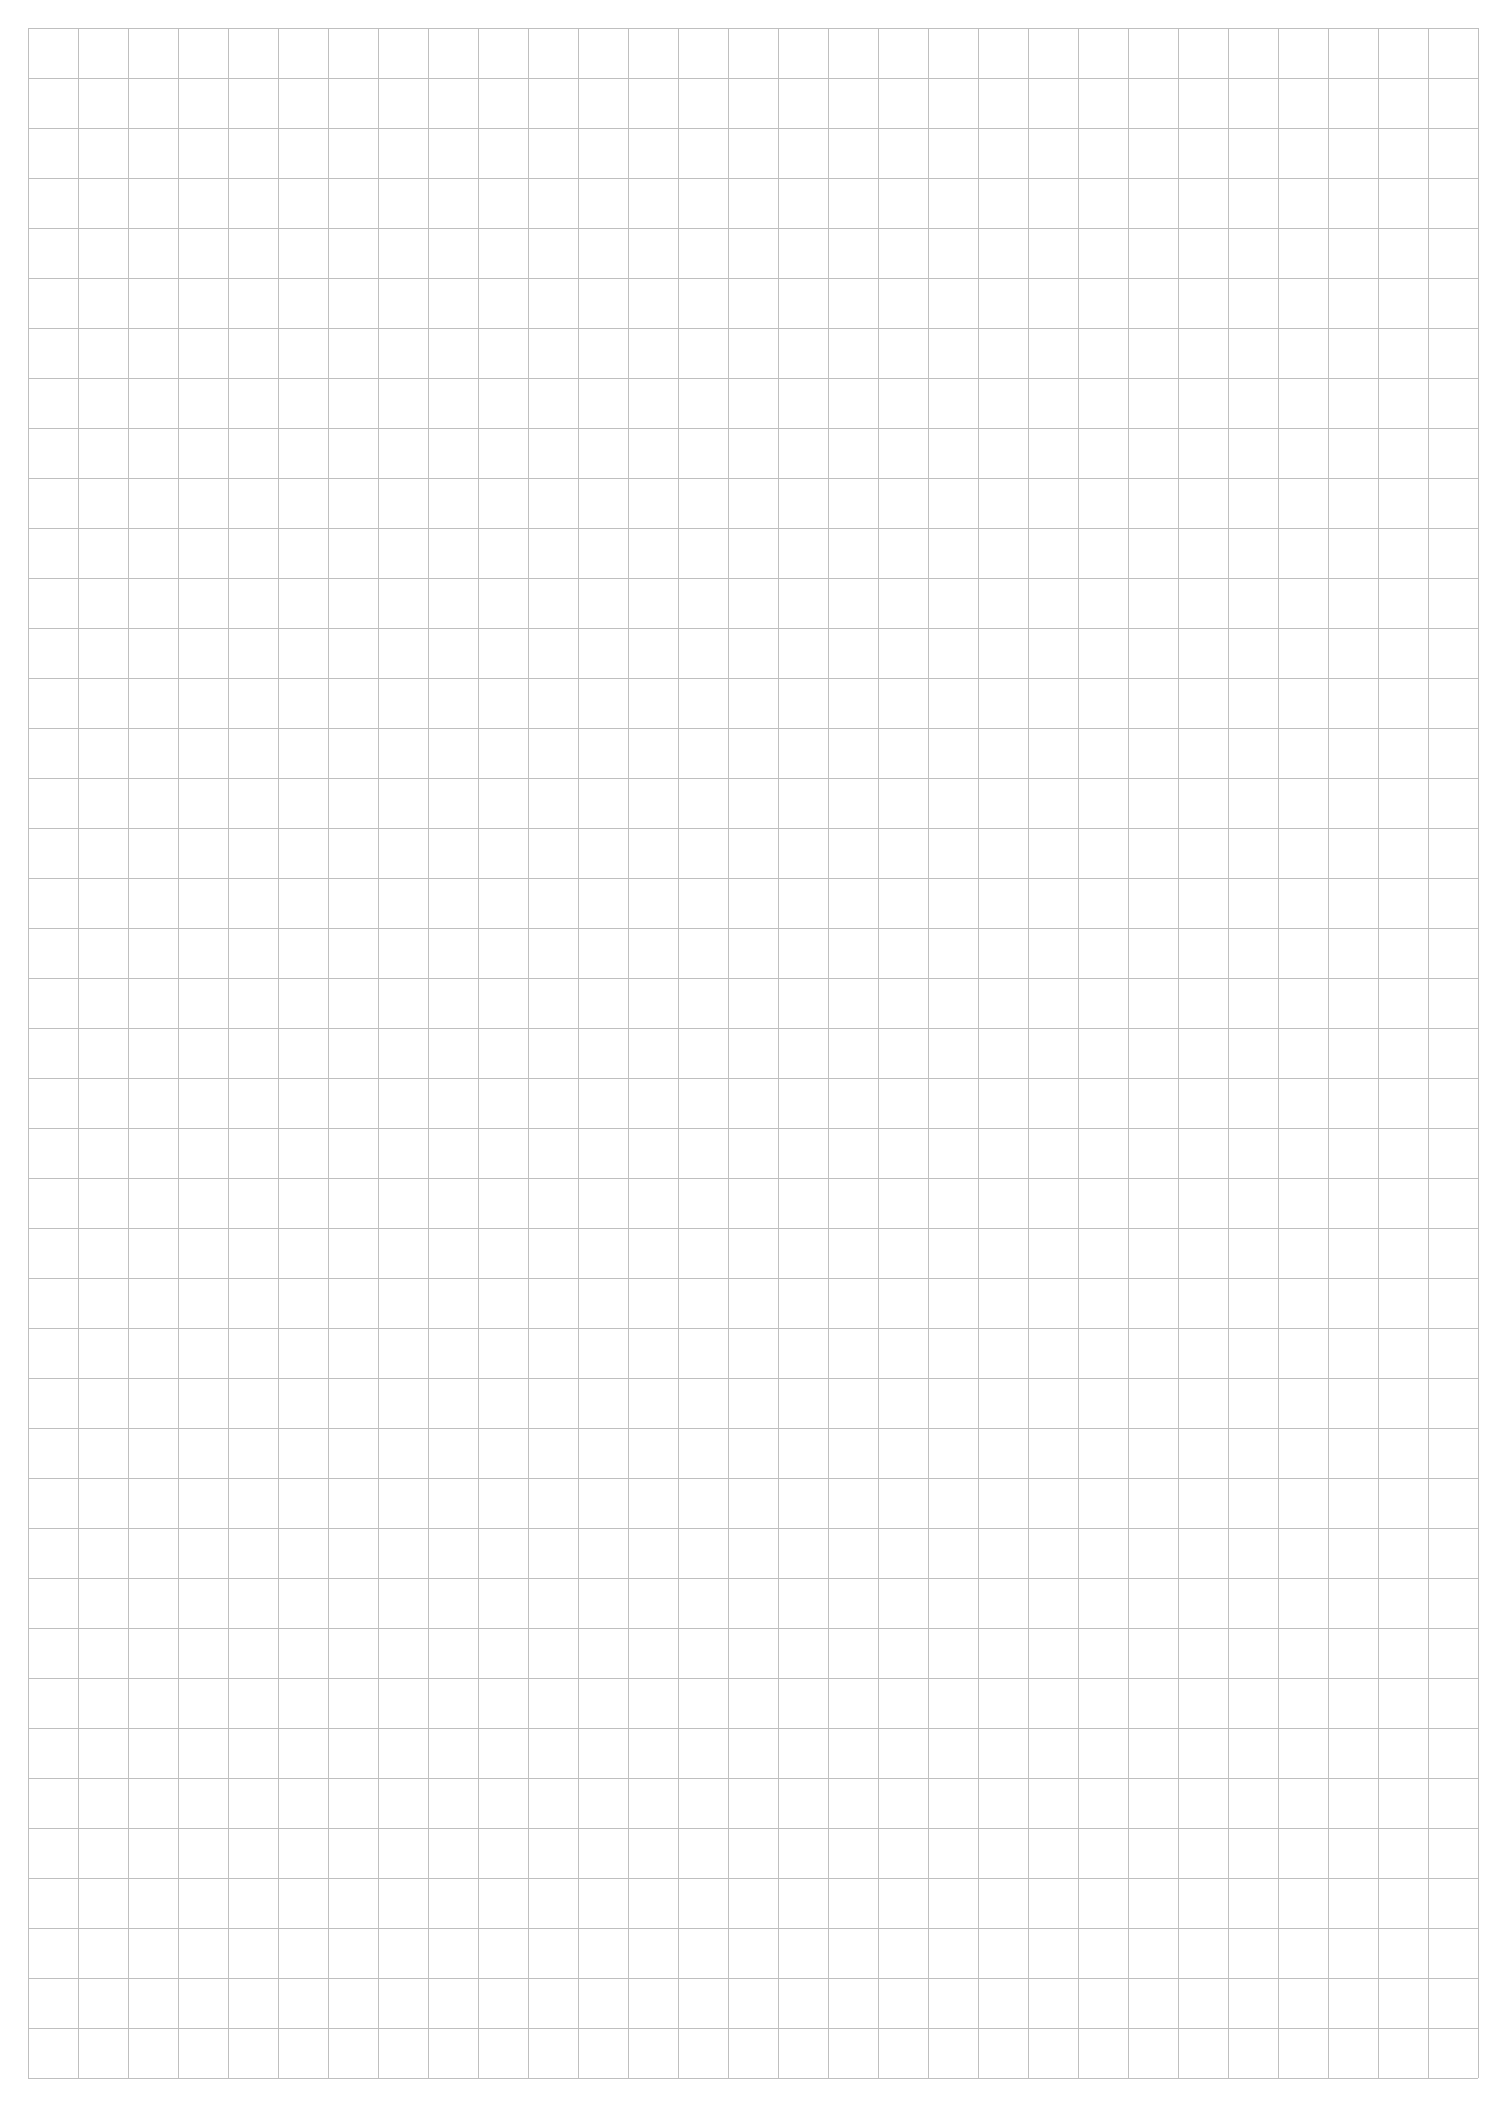
\begin{tikzpicture}[line width=0.1mm]
		\draw[color=gray!50, step=0.25in] (0,0) grid +(7.25in,10.25in);
	\end{tikzpicture}
\end{textblock*}

\begin{textblock*}{6.75in}(1in, 0.225in)
	\cbox{
		$$  Q=\frac{CD^{2.63}\left(\frac{h_L}{L}\right)^{0.54}}{279000}$$\parb
		5)  Solve the equation for $h_L$, then evaluate $h_L$ using the values $Q=135$, $C=120$, $D=202.7$ and $L=1200$
	}
\end{textblock*}


\begin{textblock*}{2.95in}(1in, 5in)
	\cbox{
    \vspace{-0.25cm}
		6) Use the Pythagorean Theorem to determine the lengths of $CE$ and $CB$
    \vspace{-0.25cm}
	}
\end{textblock*}

\begin{textblock*}{3.255in}(4.5in, 5in)  
	\cbox{
		\centering
    \vspace{-0.25cm}
    
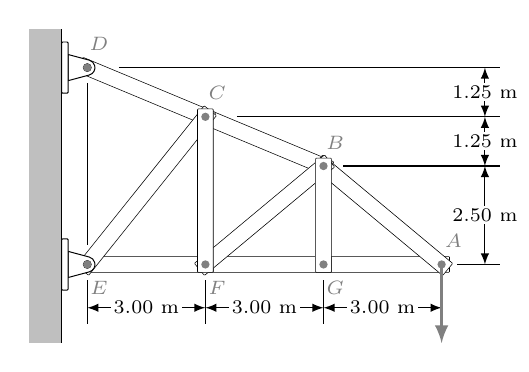
\begin{tikzpicture}



	\def\offset{0.2}
	
	\coordinate (E) at (0,0);
	\coordinate (F) at (1.5,0);
	\coordinate (G) at (3,0);
	\coordinate (A) at (4.5,0);
	\coordinate (B) at (3,1.25);
	\coordinate (C) at (1.5,1.875);
	\coordinate (D) at (0,2.5);
	\coordinate (Right) at ($ (A)+(0.75,0)$);
	\coordinate (Bottom) at ($ (A)+(0,-0.75)$);

	\filldraw[gray!50] ($(D)+(-0.325,0.5)$) rectangle ($(E)+(-.75,-1)$);
	\draw ($(D)+(-0.325,0.5)$) -- ($(E)+(-0.325,-1)$);


	\gettikzxy{(A)}{\ax}{\ay}
	\gettikzxy{(B)}{\bx}{\by}
	\gettikzxy{(C)}{\cx}{\cy}
	\gettikzxy{(D)}{\ddx}{\ddy}
	\gettikzxy{(E)}{\ex}{\ey}
	\gettikzxy{(F)}{\fx}{\fy}
	\gettikzxy{(G)}{\gx}{\gy}
	\gettikzxy{(Right)}{\rx}{\ry}
	\gettikzxy{(Bottom)}{\bbx}{\bby}

	\draw ($ (A)+(\offset,0)$) -- (\rx,\ay);
	\draw ($ (B)+(1.25*\offset,0)$) -- (\rx,\by);
	\draw ($ (C)+(2*\offset,0)$) -- (\rx,\cy);
	\draw ($ (D)+(2*\offset,0)$) -- (\rx,\ddy);
	\draw ($ (D)+(0, -\offset)$) -- (\ex,\ey+1.25*\offset cm);
	\draw ($ (E)+(0, -\offset)$) -- (\ex,\bby);
	\draw ($ (F)+(0, -\offset)$) -- (\fx,\bby);
	\draw ($ (G)+(0, -\offset)$) -- (\gx,\bby);
	\draw ($ (A)+(0, -\offset)$) -- (\ax,\bby);

	\small
	\draw[latex-latex] (\ex,\bby+\offset cm) -- node[fill=white, inner sep=0.35mm] {\scriptsize $3.00$ m}(\fx,\bby+\offset cm);
	\draw[latex-latex] (\fx,\bby+\offset cm) -- node[fill=white, inner sep=0.35mm] {\scriptsize $3.00$ m}(\gx,\bby+\offset cm);
	\draw[latex-latex] (\gx,\bby+\offset cm) -- node[fill=white, inner sep=0.35mm] {\scriptsize $3.00$ m}(\ax,\bby+\offset cm);
	\draw[latex-latex] (\rx-\offset cm,\ay) -- node[fill=white, inner sep=0.35mm] {\scriptsize $2.50$ m}(\rx-\offset cm,\by);
	\draw[latex-latex] (\rx-\offset cm,\by) -- node[fill=white, inner sep=0.35mm] {\scriptsize $1.25$ m}(\rx-\offset cm,\cy);
	\draw[latex-latex] (\rx-\offset cm,\cy) -- node[fill=white, inner sep=0.35mm] {\scriptsize $1.25$ m}(\rx-\offset cm,\ddy);
	\normalsize

	 
	 \Member{B}{C}{white}{white}{black}{0.2}{0.095}{0.2}
	 \Member{C}{D}{white}{white}{black}{0.2}{0.095}{0.2}
	 \Member{A}{G}{white}{white}{black}{0.2}{0.095}{0.2}
	 \Member{A}{B}{white}{white}{black}{0.2}{0.095}{0.2}
	 \Member{F}{G}{white}{white}{black}{0.2}{0.095}{0.2}
	 \Member{F}{E}{white}{white}{black}{0.2}{0.095}{0.2}
	 \Member{B}{F}{white}{white}{black}{0.2}{0.095}{0.2}
	 \Member{B}{G}{white}{white}{black}{0.2}{0.095}{0.2}
	 \Member{C}{E}{white}{white}{black}{0.2}{0.095}{0.2}
	 \Member{C}{F}{white}{white}{black}{0.2}{0.095}{0.2}

	\PC[-90]{D}{white}{black}{0.325}{0.125}
	\PC[-90]{E}{white}{black}{0.325}{0.125}

	\draw[very thick, gray, -latex] (A) -- +(0,-1);

	\fill[gray] (A) circle (1.5pt) node[xshift=1.5mm, yshift=3mm] {\scriptsize $A$};
	\fill[gray] (B) circle (1.5pt) node[xshift=1.5mm, yshift=3mm] {\scriptsize $B$};
	\fill[gray] (C) circle (1.5pt) node[xshift=1.5mm, yshift=3mm] {\scriptsize $C$};
	\fill[gray] (D) circle (1.5pt) node[xshift=1.5mm, yshift=3mm] {\scriptsize $D$};
	\fill[gray] (E) circle (1.5pt) node[xshift=1.5mm, yshift=-3mm] {\scriptsize $E$};
	\fill[gray] (F) circle (1.5pt) node[xshift=1.5mm, yshift=-3mm] {\scriptsize $F$};
	\fill[gray] (G) circle (1.5pt) node[xshift=1.5mm, yshift=-3mm] {\scriptsize $G$};
\pgfresetboundingbox
\draw[white] ($ (D)+ (-0.75,0.5) $) rectangle ($ (A)+(0.75,-1) $);

\end{tikzpicture}

    \vspace{-0.125cm}
	}
\end{textblock*}


%%%%%%%%%%%%%%%%%%%%%%%%%%%%%%%%%%%%%%%%%%%%%%%%%%%%%%%%%%%%%%%%%%%%%%%%%%%%%%%%%%%%%%%%%%%%%%%%%%%%
% page 3
%%%%%%%%%%%%%%%%%%%%%%%%%%%%%%%%%%%%%%%%%%%%%%%%%%%%%%%%%%%%%%%%%%%%%%%%%%%%%%%%%%%%%%%%%%%%%%%%%%%%
.\newpage

\begin{textblock*}{7.25in}(1in, 0.4in)
  % \textblockcolor{pink}
	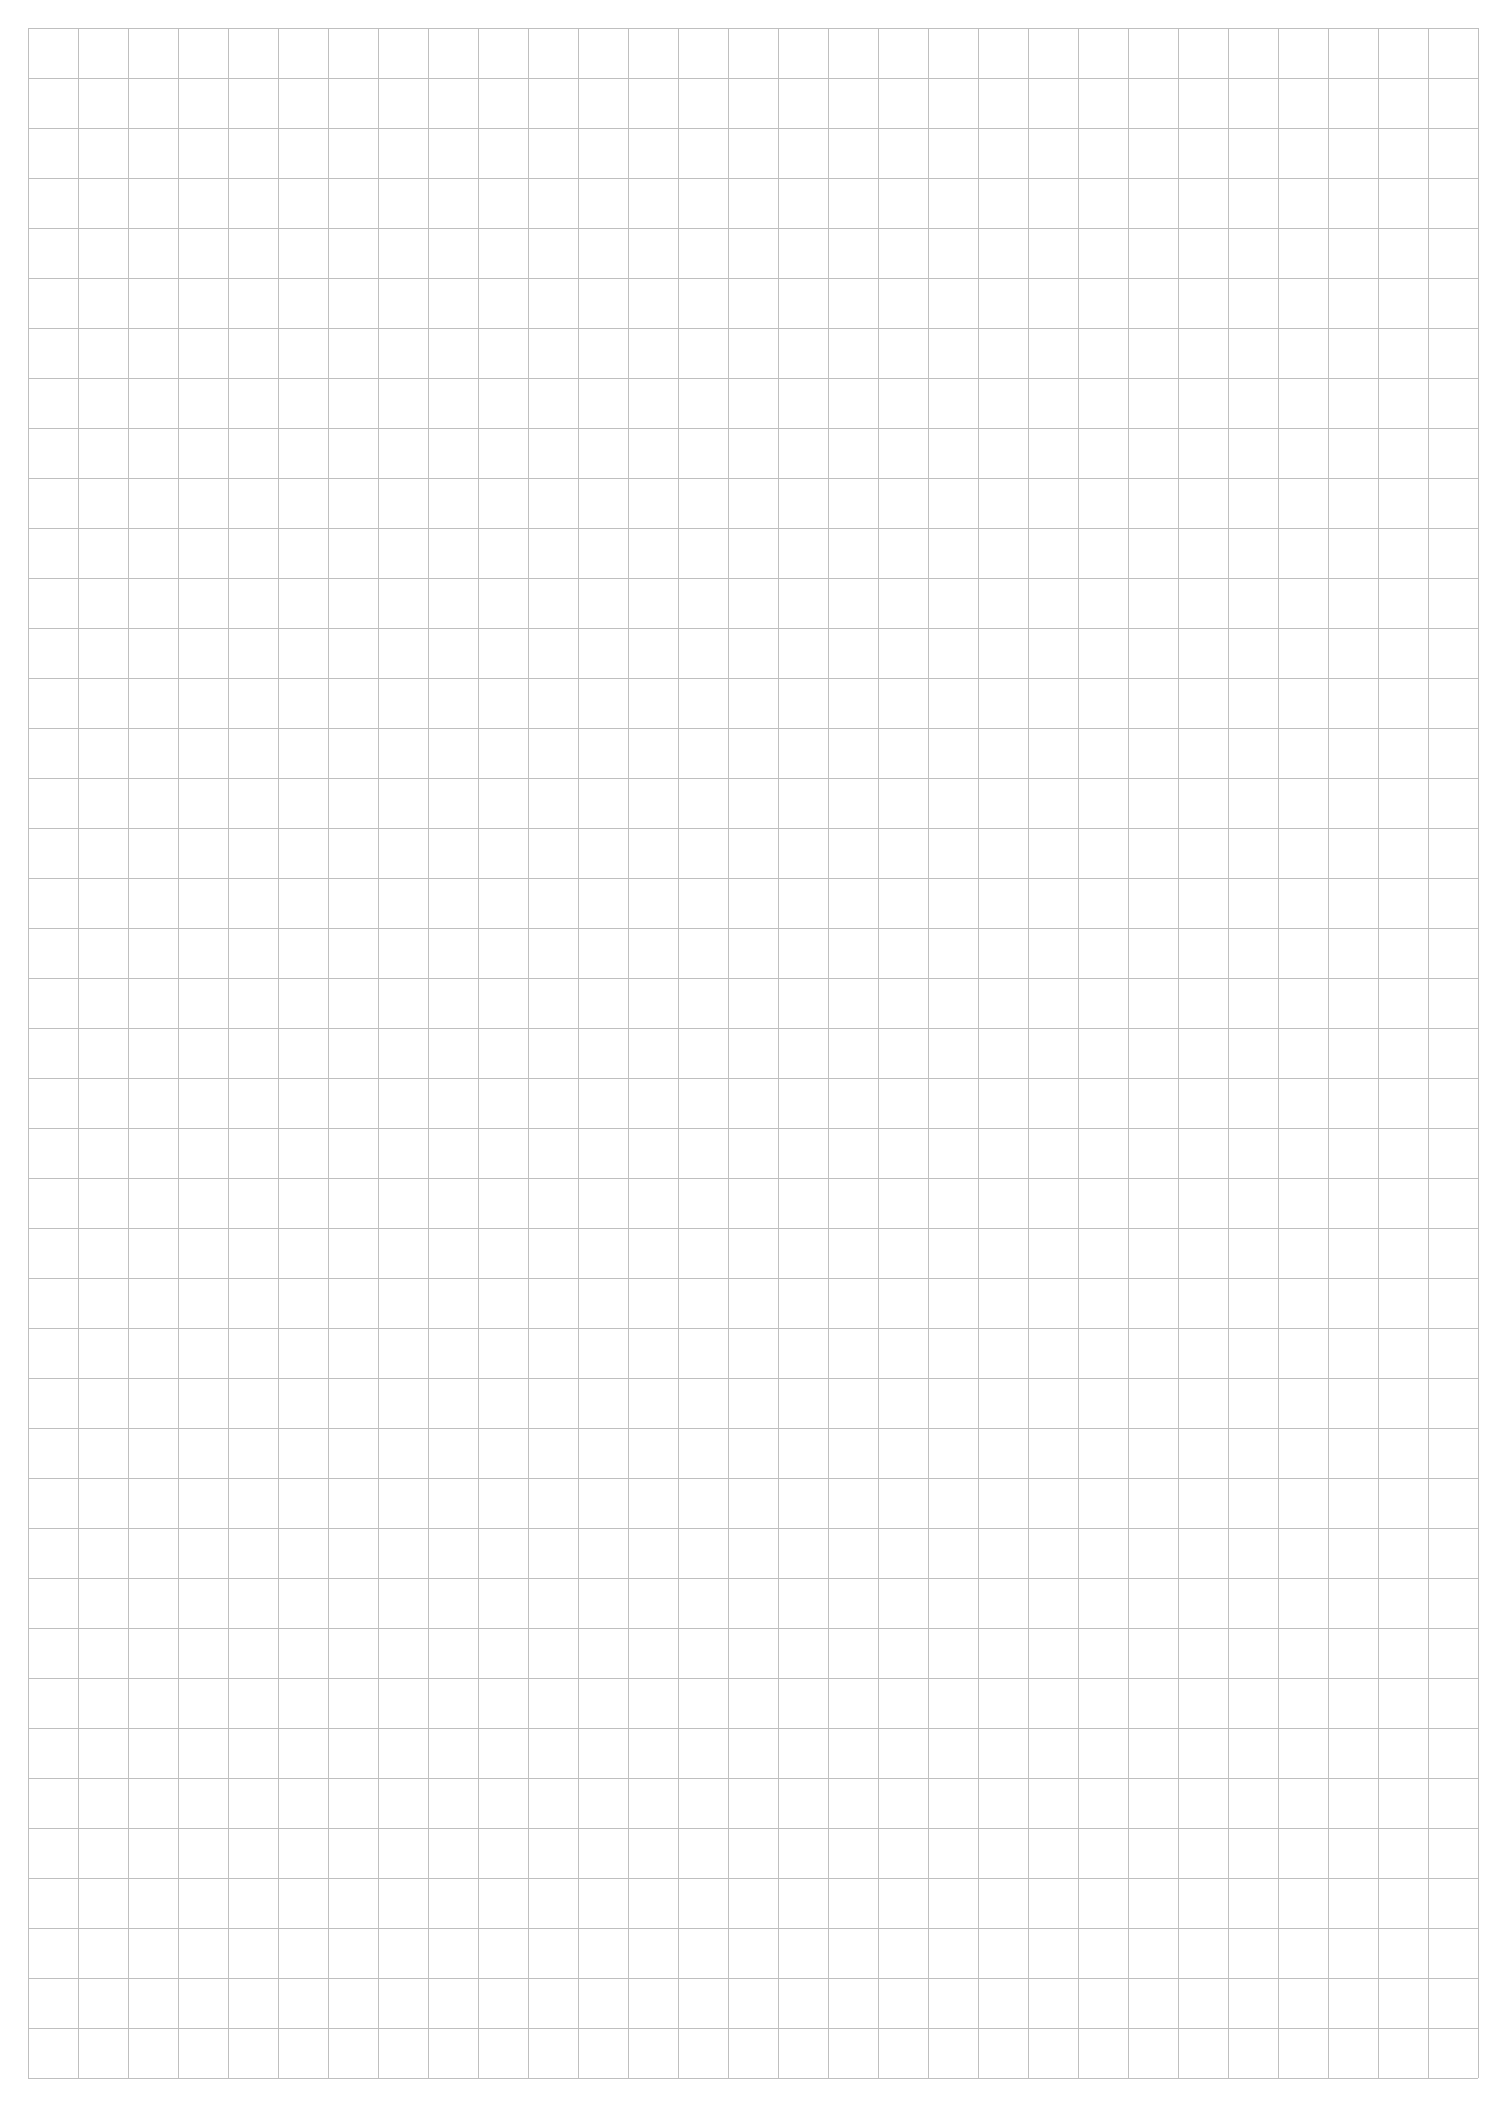
\begin{tikzpicture}[line width=0.1mm]
		\draw[color=gray!50, step=0.25in] (0,0) grid +(7.25in,10.25in);
	\end{tikzpicture}
\end{textblock*}


\begin{textblock*}{6.75in}(1in, 0.225in)
	\cbox{
    \vspace{-0.25cm}
		7) Use the tangent function to calculate $\angle CEF$
    \vspace{-0.375cm}
	}
\end{textblock*}

\begin{textblock*}{6.75in}(1in, 2.5in)
	\cbox{
    \vspace{-0.25cm}
		8) Use $\angle CEF$ just found and the sine rule to verify the length of $CE$ found in 1) above.
    \vspace{-0.375cm}
	}
\end{textblock*}

\begin{textblock*}{6.75in}(1in, 5in)
	\cbox{
    \vspace{-0.25cm}
		9) Use the cosine function and the length of $BC$ found earlier to calculate the angle between $BC$ and the horizontal.
    \vspace{-0.25cm}
	}
\end{textblock*}


\begin{textblock*}{6.75in}(1in, 7.5in)
	\cbox{
    \vspace{-0.25cm}
		10) Use the tangent function to verify the previous result.
    \vspace{-0.5cm}
	}
\end{textblock*}

%%%%%%%%%%%%%%%%%%%%%%%%%%%%%%%%%%%%%%%%%%%%%%%%%%%%%%%%%%%%%%%%%%%%%%%%%%%%%%%%%%%%%%%%%%%%%%%%%%%%
% page 4
%%%%%%%%%%%%%%%%%%%%%%%%%%%%%%%%%%%%%%%%%%%%%%%%%%%%%%%%%%%%%%%%%%%%%%%%%%%%%%%%%%%%%%%%%%%%%%%%%%%%
.\newpage

\begin{textblock*}{7.25in}(1in, 0.375in)
  % \textblockcolor{pink}
	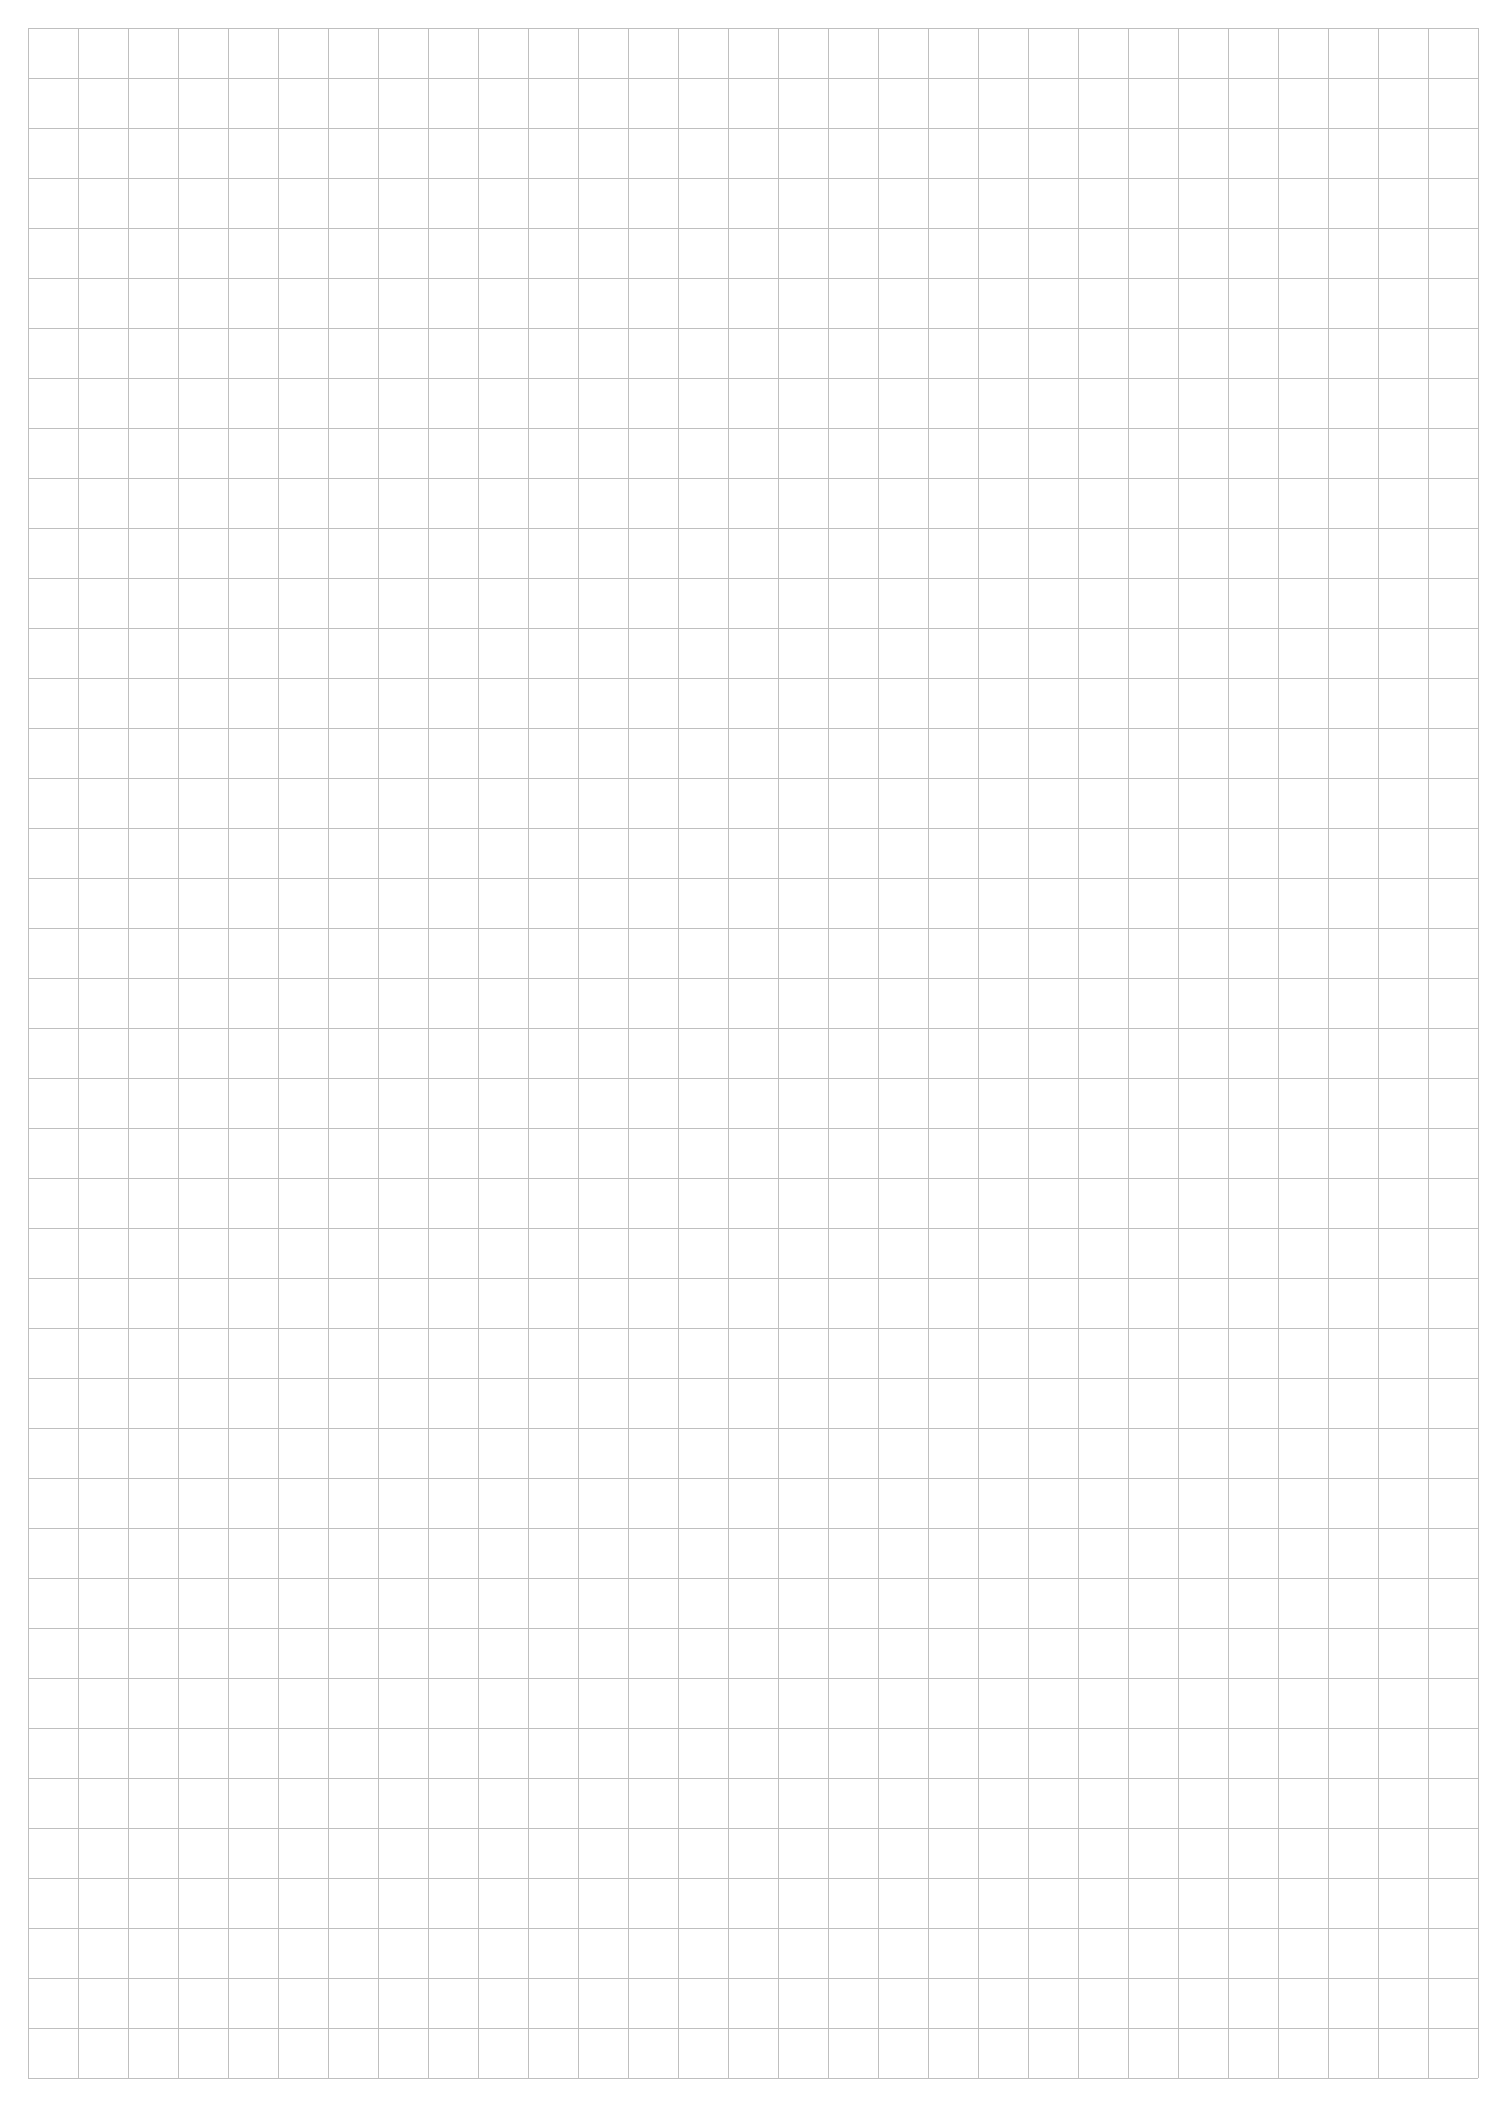
\begin{tikzpicture}[line width=0.1mm]
		\draw[color=gray!50, step=0.25in] (0,0) grid +(7.25in,10.25in);
	\end{tikzpicture}
\end{textblock*}

\begin{textblock*}{2.5in}(5.25in, 0.225in)
	\cbox{
		\centering
		% !TEX root = ../../Beamer/statikz/statikz.tex


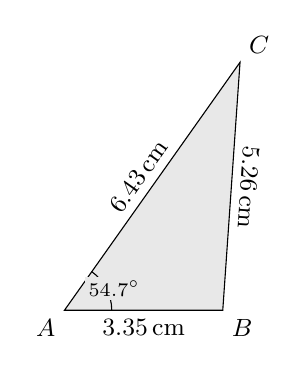
\begin{tikzpicture}[scale=0.6]

	\coordinate (A) at (0,0);
	\coordinate (B) at ($ (A)+(3.35, 0)$);
	\coordinate (C) at ($ (A)+(54.7:6.43)$);
	
  

	\small
	\filldraw[fill=Gainsboro!65, draw=black] (A) -- (B) --  (C) --  cycle;
  
	\path (A) -- (C) node[midway, sloped, above] {$6.43\,$cm};
	\path (C) -- (B) node[midway, sloped, above, rotate=180] {$5.26\,$cm};
	\path (A) -- (B) node[midway, sloped, below] {$3.35\,$cm};
	\draw[below right] (B) node {$B$};
	\draw[below left] (A) node {$A$};
	\draw[above right] (C) node {$C$};

	\draw ($ (A)+(54.7:1) $) arc (54.7:0:1)node[midway, fill=Gainsboro!65, inner sep=0.5mm,xshift=1mm] {\scriptsize $ 54.7\deg $};
  

	% \node[xshift=-0.5cm, yshift=0.15cm] at (C) {$\theta $};



\end{tikzpicture}

	}
\end{textblock*}

\begin{textblock*}{3.7in}(1in, 0.225in)
	\cbox{
    \vspace{-0.25cm}
		11) Using the sine rule, find $\angle ACB$.
    \vspace{-0.375cm}
	}
\end{textblock*}

\begin{textblock*}{6.75in}(1in, 2.5in)
	\cbox{
    \vspace{-0.25cm}
		12) Using the sine rule, find $\angle ABC$.
    \vspace{-0.5cm}
	}
\end{textblock*}

\begin{textblock*}{6.75in}(1in, 4.5in)
	\cbox{
    \vspace{-0.25cm}
		13) Sum the interior angles of the triangle.
    \vspace{-0.5cm}
	}
\end{textblock*}

\begin{textblock*}{3.95in}(1in, 6.5in)
	\cbox{
    \vspace{-0.25cm}
		14) Using the cosine rule, determine $\angle ABC$ \lb
		15) Compare the value for $\angle ABC$ with the value calculated earlier.
    \vspace{-0.25cm}
	}
\end{textblock*}

\begin{textblock*}{2.225in}(5.525in, 6.5in)
	\cbox{
		\centering
		% !TEX root = ../../Beamer/statikz/statikz.tex


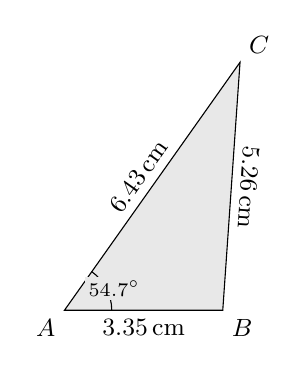
\begin{tikzpicture}[scale=0.6]

	\coordinate (A) at (0,0);
	\coordinate (B) at ($ (A)+(3.35, 0)$);
	\coordinate (C) at ($ (A)+(54.7:6.43)$);
	
  

	\small
	\filldraw[fill=Gainsboro!65, draw=black] (A) -- (B) --  (C) --  cycle;
  
	\path (A) -- (C) node[midway, sloped, above] {$6.43\,$cm};
	\path (C) -- (B) node[midway, sloped, above, rotate=180] {$5.26\,$cm};
	\path (A) -- (B) node[midway, sloped, below] {$3.35\,$cm};
	\draw[below right] (B) node {$B$};
	\draw[below left] (A) node {$A$};
	\draw[above right] (C) node {$C$};

	\draw ($ (A)+(54.7:1) $) arc (54.7:0:1)node[midway, fill=Gainsboro!65, inner sep=0.5mm,xshift=1mm] {\scriptsize $ 54.7\deg $};
  

	% \node[xshift=-0.5cm, yshift=0.15cm] at (C) {$\theta $};



\end{tikzpicture}

	}
\end{textblock*}


%%%%%%%%%%%%%%%%%%%%%%%%%%%%%%%%%%%%%%%%%%%%%%%%%%%%%%%%%%%%%%%%%%%%%%%%%%%%%%%%%%%%%%%%%%%%%%%%%%%%
% page 5
%%%%%%%%%%%%%%%%%%%%%%%%%%%%%%%%%%%%%%%%%%%%%%%%%%%%%%%%%%%%%%%%%%%%%%%%%%%%%%%%%%%%%%%%%%%%%%%%%%%%
.\newpage

\begin{textblock*}{7.25in}(1in, 0.375in)
  % \textblockcolor{pink}
	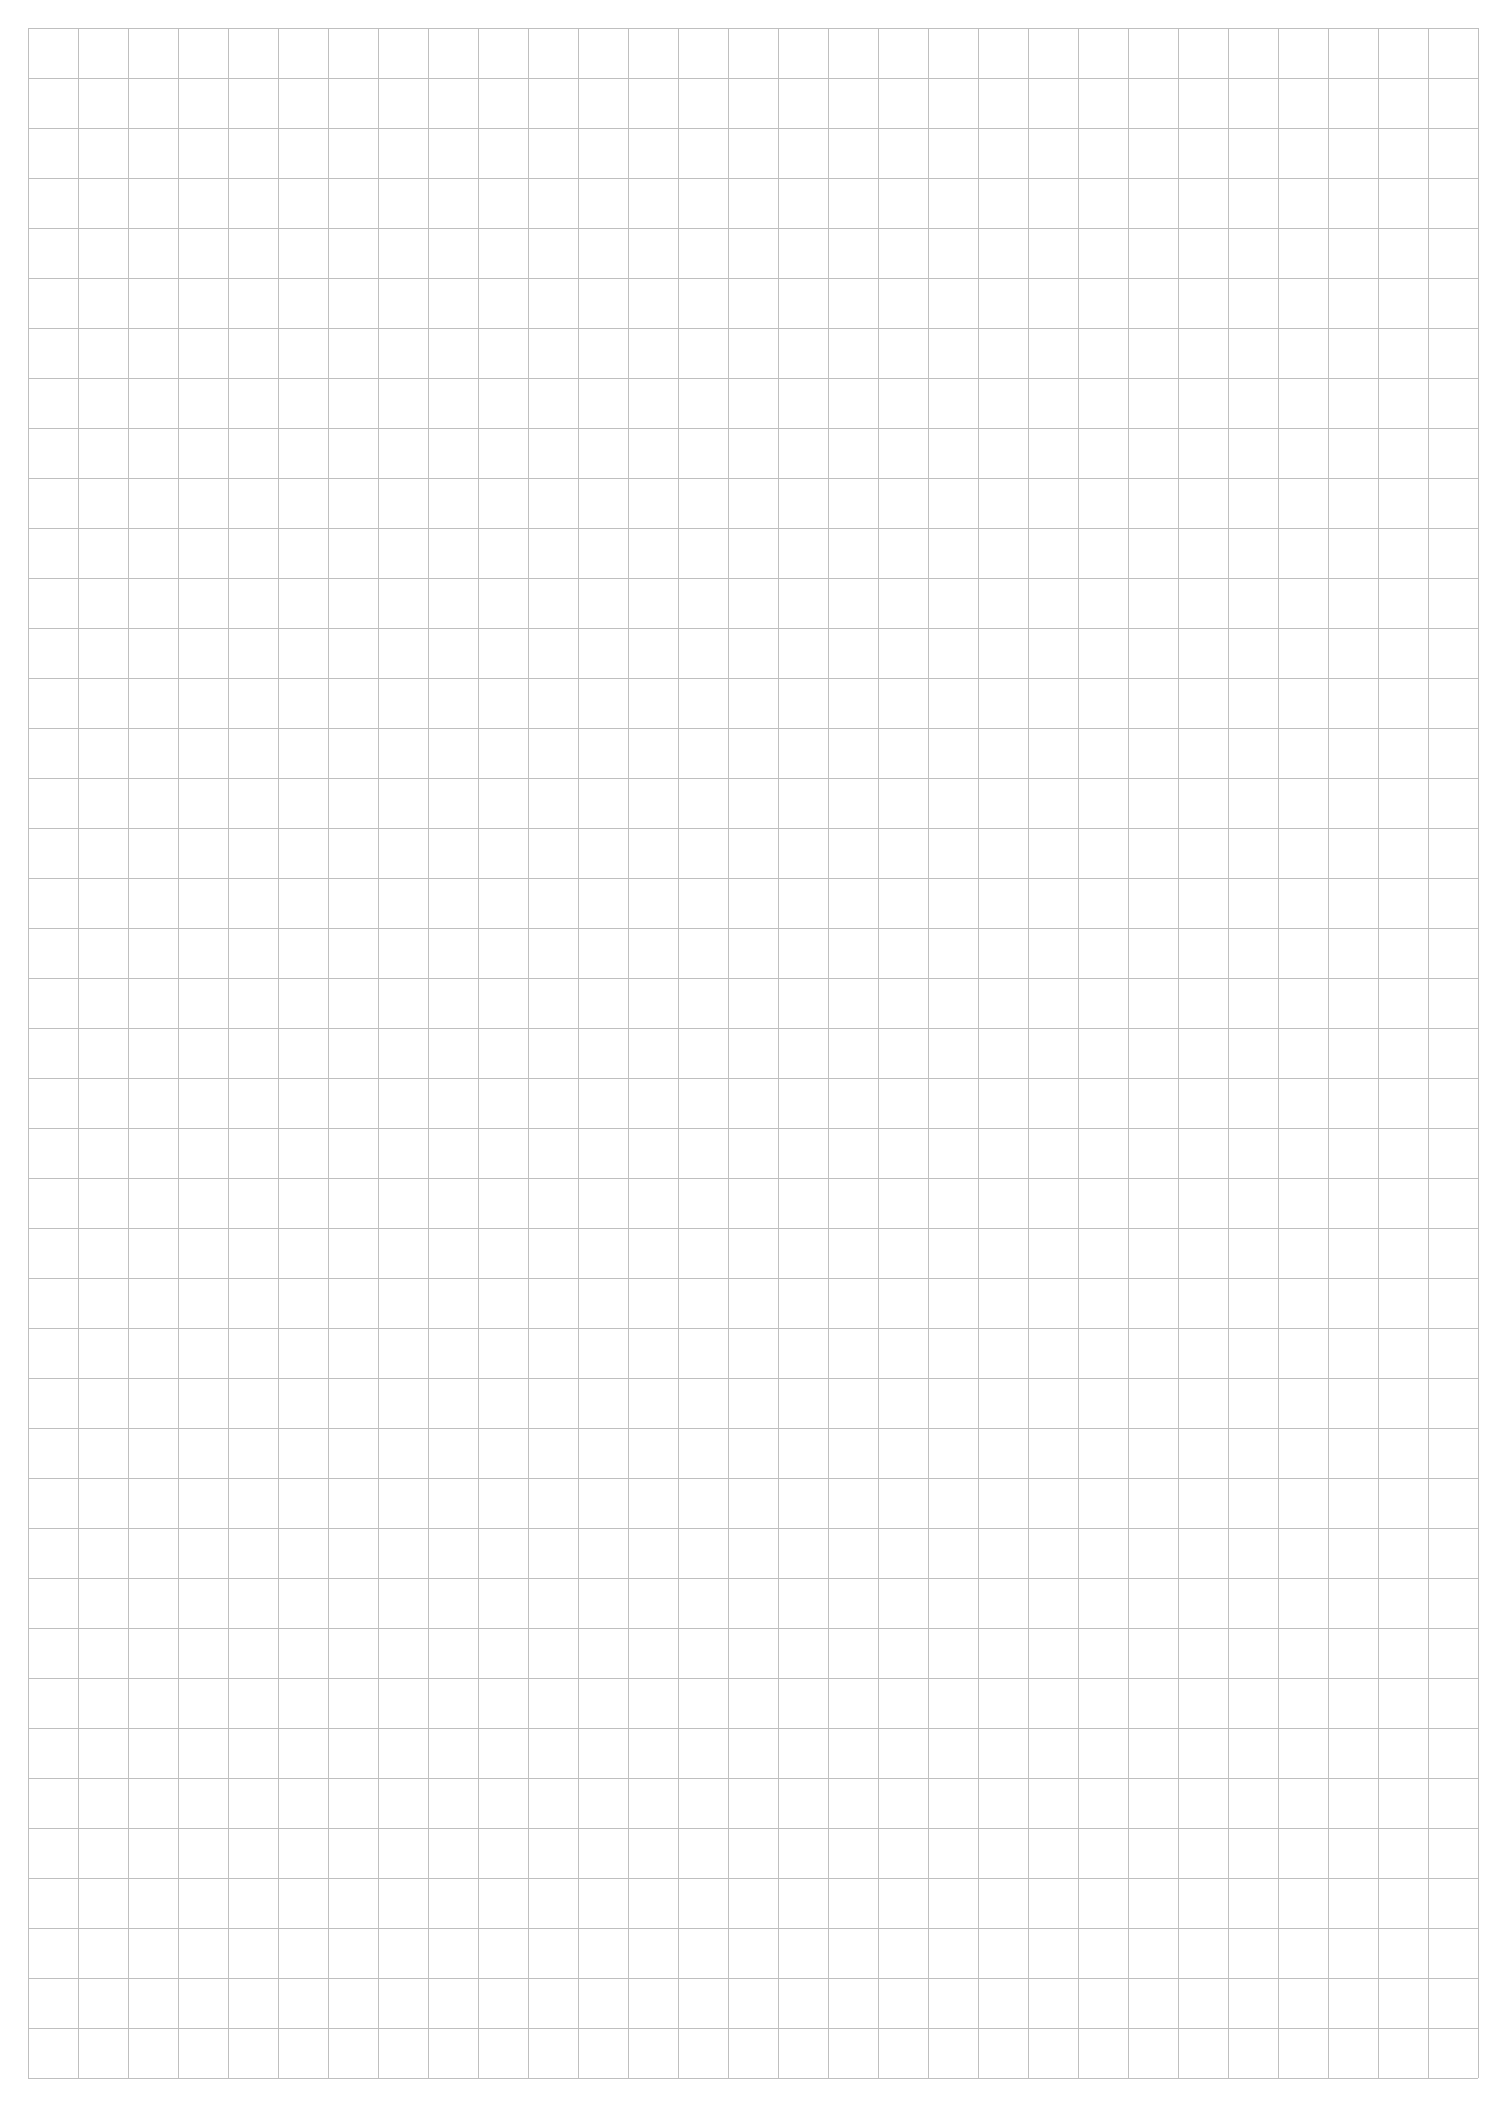
\begin{tikzpicture}[line width=0.1mm]
		\draw[color=gray!50, step=0.25in] (0,0) grid +(7.25in,10.25in);
	\end{tikzpicture}
\end{textblock*}



\begin{textblock*}{2.725in}(5.025in, 0.225in)
	\cbox{
    \vspace{-0.25cm}
		\centering
		


\scalebox{0.75}{
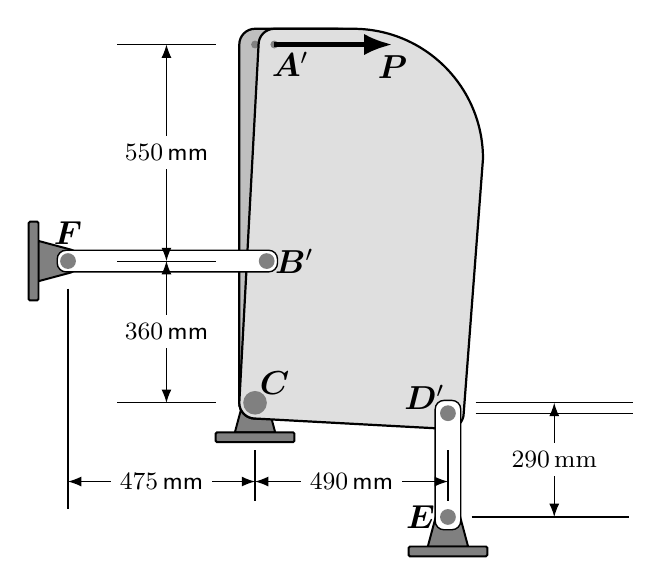
\begin{tikzpicture}[scale=1]

	\coordinate (C) at (0,0);
	\coordinate (B) at ($ (C)+(90:1.8)  $);
	\coordinate (BB) at ($ (B)+(0:0.148)  $);
	\coordinate (A) at ($ (B)+(90:2.75) $);
	\coordinate (AA) at ($ (A)+(0:0.245) $);
  \coordinate (D) at ($ (C)+(0:2.45) $);
  \coordinate (DD) at ($ (D)+(-90:.132) $);
	\coordinate (E) at ($ (D)+(-90:1.45) $);
	\coordinate (F) at ($ (B)+(180:2.375) $);
	\def\d{0.2cm}

	\gettikzxy{(A)}{\ax}{\ay}
	\gettikzxy{(AA)}{\aax}{\aay}
  \gettikzxy{(B)}{\bx}{\by}
  \gettikzxy{(BB)}{\bbx}{\bby}
  \gettikzxy{(C)}{\cx}{\cy}
  \gettikzxy{(D)}{\ddx}{\ddy}
  \gettikzxy{(DD)}{\dddx}{\dddy}
  \gettikzxy{(E)}{\ex}{\ey}
  \gettikzxy{(F)}{\fx}{\fy}

	\PC[270]{F}{gray}{black}{0.5}{0.25}
	\PC{E}{gray}{black}{0.5}{0.25}
	\PC{C}{gray}{black}{0.5}{0.25}

	\small


		\filldraw[thick, fill=gray!50, draw=black] (\cx-\d, \cy)--(\cx-\d, \ay)arc(180:90:\d)--+(1,0)arc(90:0:1.65)--(\ddx+\d, \ddy)arc(0:-90:\d)--(\cx, \cy-\d)arc(270:180:\d);


		
		\draw[thin] (\ddx+0.35cm, \ddy) -- +(2,0);
		\draw[Latex-Latex] (\ddx+1.35cm,\ddy) -- node[fill=white] { $290\,\text{mm}$}(\ddx+1.35cm,\ey);
	
		\fill [gray] (B) circle (0.1cm) node[black, xshift=0.3cm] {\large $\bm B$};	
		\fill [gray] (A) circle (0.05cm) node[black, xshift=0.2cm, yshift=-0.25cm] {\large $\bm A$};
		\fill [gray] (D) circle (0.1cm) node[black, xshift=-0.3cm, yshift=0.2cm] {\large $\bm D$};



		\filldraw[thick, gray!25, draw=black] (\cx-\d, \cy)--(\aax-\d, \aay)arc(180:90:\d)--+(1,0)arc(90:0:1.65)--(\dddx+\d, \dddy)arc(0:-90:\d)--(\cx, \cy-\d)arc(270:180:\d);
		% \draw[Latex-Latex] (\dddx+1.35cm,\dddy) -- node[fill=white] { $290\,\mathsf{mm}-\delta_{DE}$}(\ddx+1.35cm,\ey);
		\draw[thin] (\dddx+0.35cm, \dddy) -- +(2,0);

		\Member{F}{BB}{white}{white}{black}{0.275}{1.125}{0.5}
		\Member{DD}{E}{white}{white}{black}{0.325}{1.125}{0.5}
		
		\fill [gray] (BB) circle (0.1cm) node[black, xshift=0.35cm] {\large $\bm B'$};
		\fill [gray] (AA) circle (0.05cm) node[black, xshift=0.2cm, yshift=-0.25cm] {\large $\bm A'$};
		\fill [gray] (DD) circle (0.1cm) node[black, xshift=-0.3cm, yshift=0.2cm] {\large $\bm D'$};
		\draw[-Latex, ultra thick, black] (AA)--+(1.5,0)node[black, below]{\large $\bm P$};



	\draw[Latex-Latex] (\cx-1.125cm,\ddy) -- node[fill=white] { $360\,\mathsf{mm}$}(\cx-1.125cm,\by);
	\draw[Latex-Latex] (\cx-1.125cm,\ay) -- node[fill=white] { $550\,\mathsf{mm}$}(\cx-1.125cm,\by);
	\draw[Latex-Latex] (\fx,\cy-1cm) -- node[fill=white] { $475\,\mathsf{mm}$}(\cx,\cy-1cm);
	\draw[Latex-Latex] (\cx,\cy-1cm) -- node[fill=white] { $490\,\mathsf{mm}$}(\ddx,\cy-1cm);

	\draw[thin] (\ax-0.5cm, \ay) -- +(-1.25, 0);
	\draw[thin] (\bx-0.5cm, \by) -- +(-1.25, 0);
	\draw[thin] (\cx-0.5cm, \cy) -- +(-1.25, 0);
	\draw[thin] (\cx, \cy-0.6cm) -- +(0, -0.65);
	\draw[thin] (\ddx, \ddy-0.6cm) -- +(0, -0.65);
	\draw[thin] (\ex+0.3cm, \ey) -- +(2,0);
	\draw[thin] (\fx, \fy-0.35cm) -- (\fx, \cy-1.35cm);
	
	\large 
	\fill [gray] (E) circle (0.1cm) node[black, xshift=-0.35cm] {$\bm E$};
	\fill [gray] (F) circle (0.1cm) node[black, yshift=0.35cm] {$\bm F$};
	\fill [gray] (C) circle (0.15cm) node[black, xshift=0.25cm, yshift=0.25cm] {\large $\bm C$};
	



\end{tikzpicture}
}
    \vspace{-0.25cm}
	}
\end{textblock*}

\begin{textblock*}{3.475in}(1in, 0.225in)
	\cbox{
    \vspace{-0.25cm}
		$ABCD$ is a rigid (i.e., it does not deform) plate, pinned at $C$. \parm
		When horizontal force $P$ is applied at $A$, $ABCD$ rotates about $C$ and $A$ deflects 2.45~mm horizontally rightwards. \parm
		Assume that $BF$ remains horizontal and that $DE$ remains vertical.\parm
		16) Determine $\delta_{BF}$, the change in length of $BF$. \parm
		17) Determine $\delta_{DE}$, the change in length of $DE$.
    \vspace{-0.25cm}
	}
\end{textblock*}

\begin{textblock*}{1.75in}(6in, 5.25in)
	\cbox{
    \vspace{-0.25cm}
		\centering
		\input{../../pikz/01MathReview/math09handout}
    \vspace{-0.5cm}
	}
\end{textblock*}

\begin{textblock*}{4.45in}(1in, 5.25in)
	\cbox{
    \vspace{-0.25cm}
		18) Show that right triangles $\triangle ABC$, $\triangle ABD$ and $\triangle ACD$ all have the same angles (i.e. they are all similar).
    \vspace{-0.25cm}
	}
\end{textblock*}

\begin{textblock*}{6.75in}(1in, 8.5in)
	\cbox{
    \vspace{-0.25cm}
		19) Given that $AC=100\text{ mm}$ and $AD=65\text{ mm}$, determine $\angle ACD$ and $\angle ABD$.
    \vspace{-0.5cm}
	}
\end{textblock*}

%%%%%%%%%%%%%%%%%%%%%%%%%%%%%%%%%%%%%%%%%%%%%%%%%%%%%%%%%%%%%%%%%%%%%%%%%%%%%%%%%%%%%%%%%%%%%%%%%%%%
% page 6
%%%%%%%%%%%%%%%%%%%%%%%%%%%%%%%%%%%%%%%%%%%%%%%%%%%%%%%%%%%%%%%%%%%%%%%%%%%%%%%%%%%%%%%%%%%%%%%%%%%%
.\newpage

\begin{textblock*}{7.25in}(1in, 0.375in)
  % \textblockcolor{pink}
	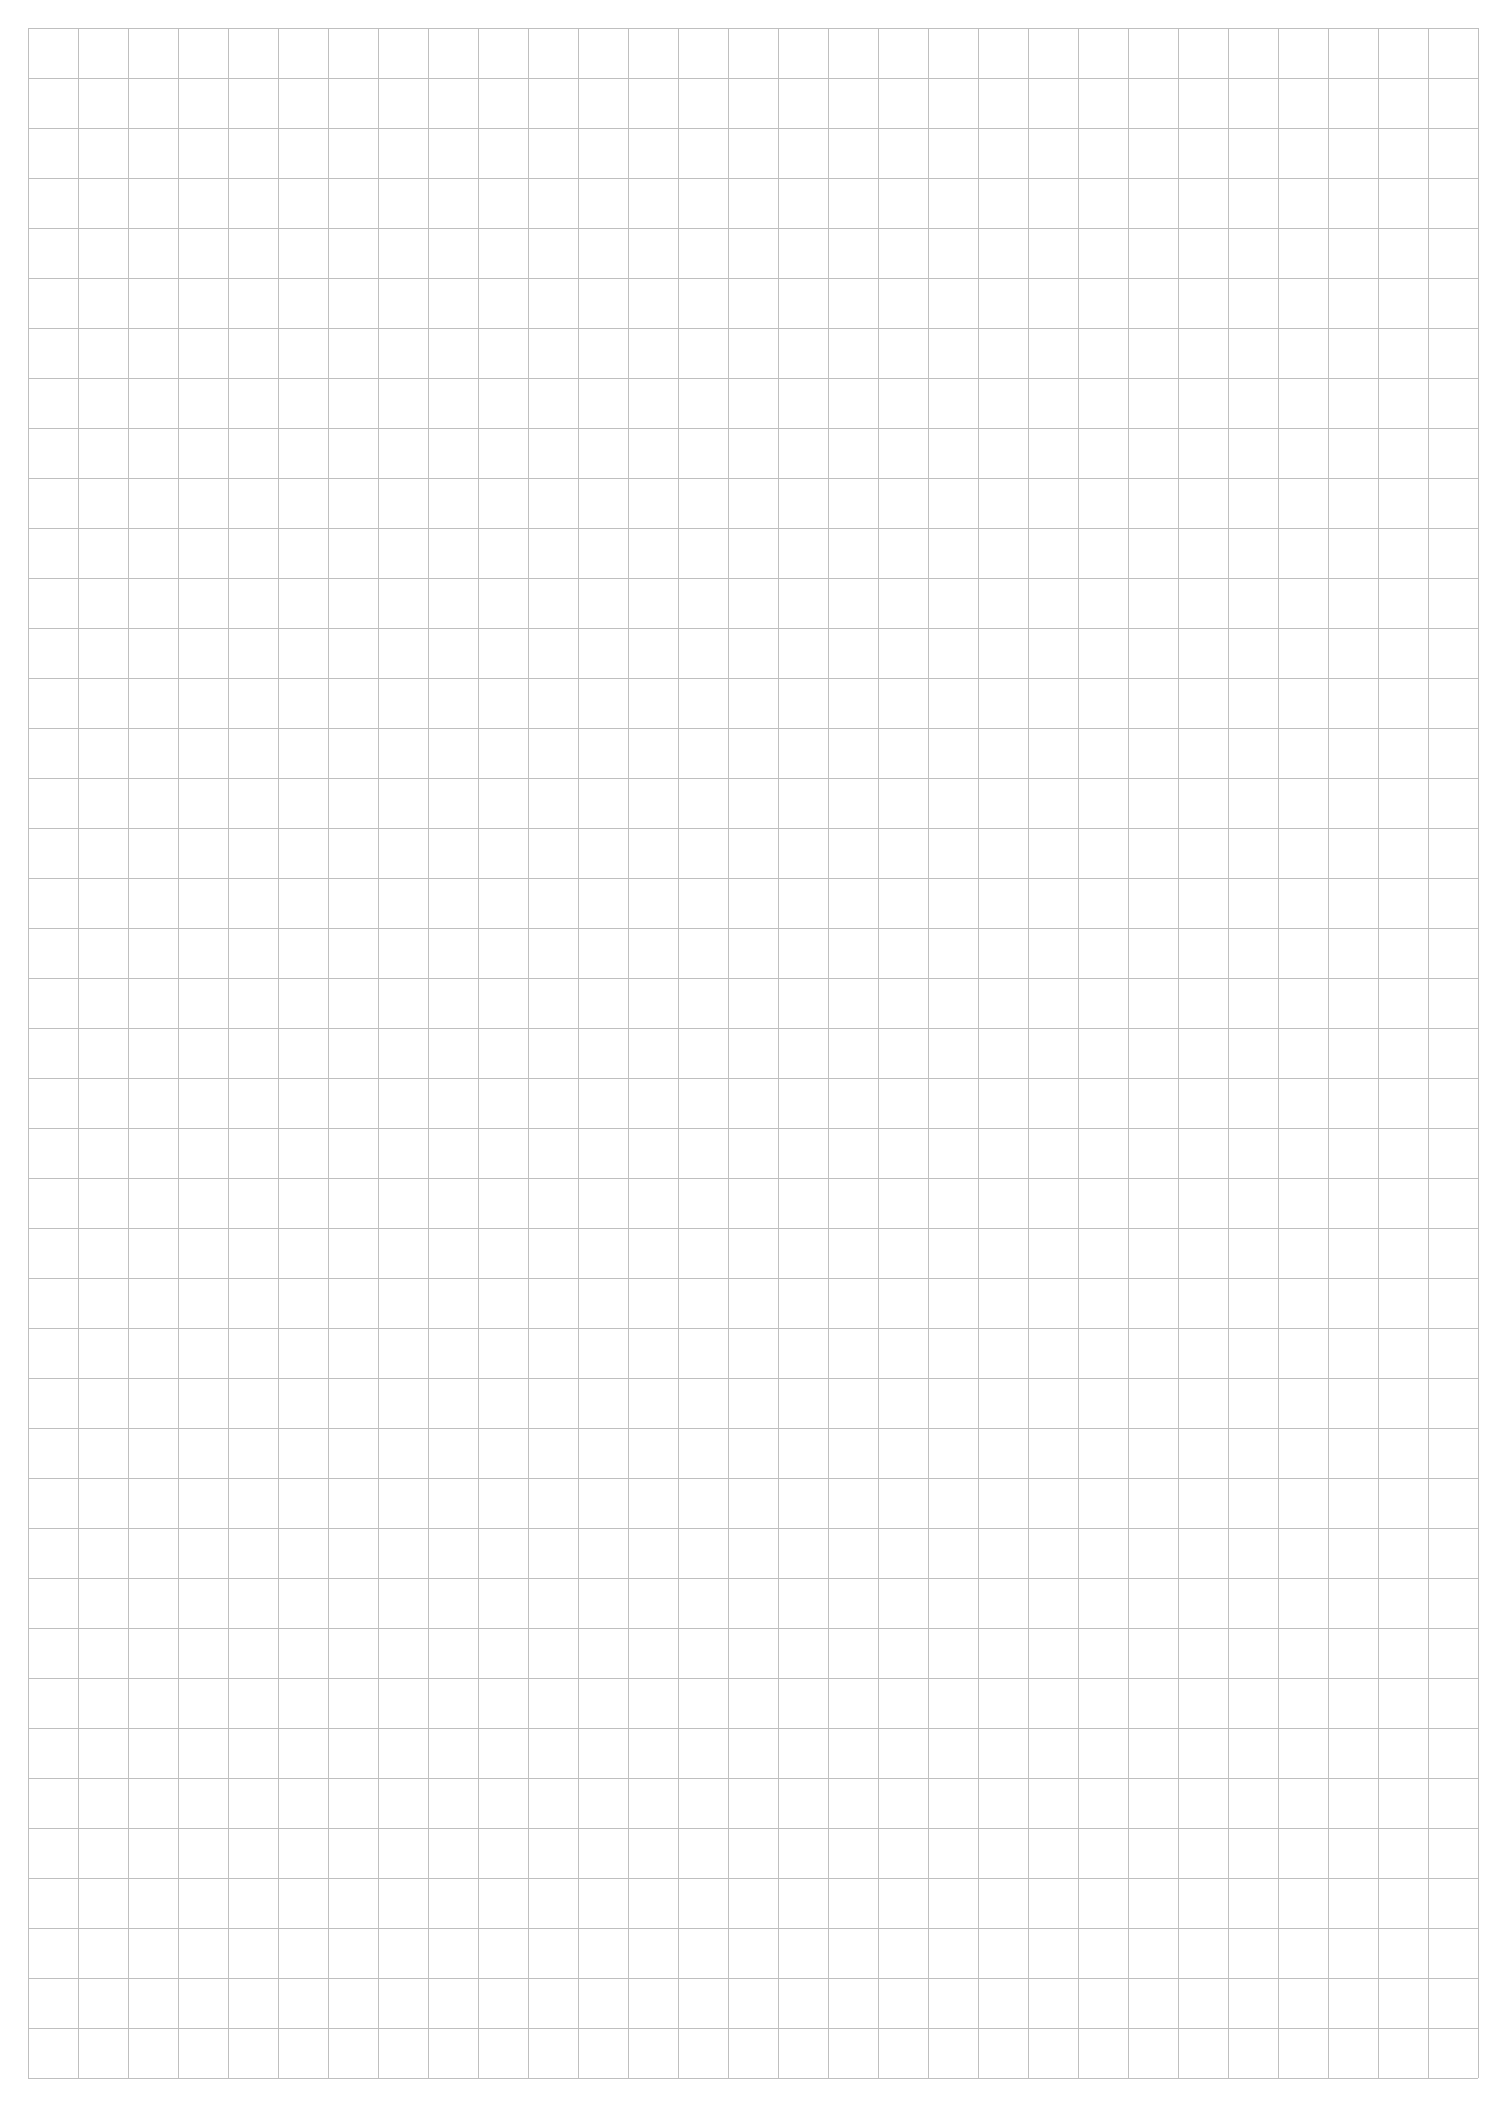
\begin{tikzpicture}[line width=0.1mm]
		\draw[color=gray!50, step=0.25in] (0,0) grid +(7.25in,10.25in);
	\end{tikzpicture}
\end{textblock*}


\begin{textblock*}{6.75in}(1in, 0.225in)
	\cbox{
    \vspace{-0.25cm}
		20) Find the remaining lengths: $AB$, $BD$ and $CD$.
    \vspace{-0.5cm}
	}
\end{textblock*}

\begin{textblock*}{6.75in}(1in, 3in)
	\cbox{
    \vspace{-0.25cm}
		21) Verify the lengths found above by using the Pythagorean Theorem on $\triangle ABC$
    \vspace{-0.5cm}
	}
\end{textblock*}

\begin{textblock*}{2.75in}(5in, 4.5in)
	\cbox{
		\centering
		\input{../../pikz/01MathReview/math10handout}
	}
\end{textblock*}

\begin{textblock*}{3.44in}(1in, 4.5in)
	\cbox{
    \vspace{-0.25cm}
		22) Find $\theta_{AC}$.\qquad\qquad\qquad\qquad
		23) Find $\theta_{BC}$.
    \vspace{-0.5cm}
	}
\end{textblock*}


%%%%%%%%%%%%%%%%%%%%%%%%%%%%%%%%%%%%%%%%%%%%%%%%%%%%%%%%%%%%%%%%%%%%%%%%%%%%%%%%%%%%%%%%%%%%%%%%%%%%
% page 7
%%%%%%%%%%%%%%%%%%%%%%%%%%%%%%%%%%%%%%%%%%%%%%%%%%%%%%%%%%%%%%%%%%%%%%%%%%%%%%%%%%%%%%%%%%%%%%%%%%%%
.\newpage
\begin{textblock*}{7.25in}(1in, 0.375in)
  % \textblockcolor{pink}
	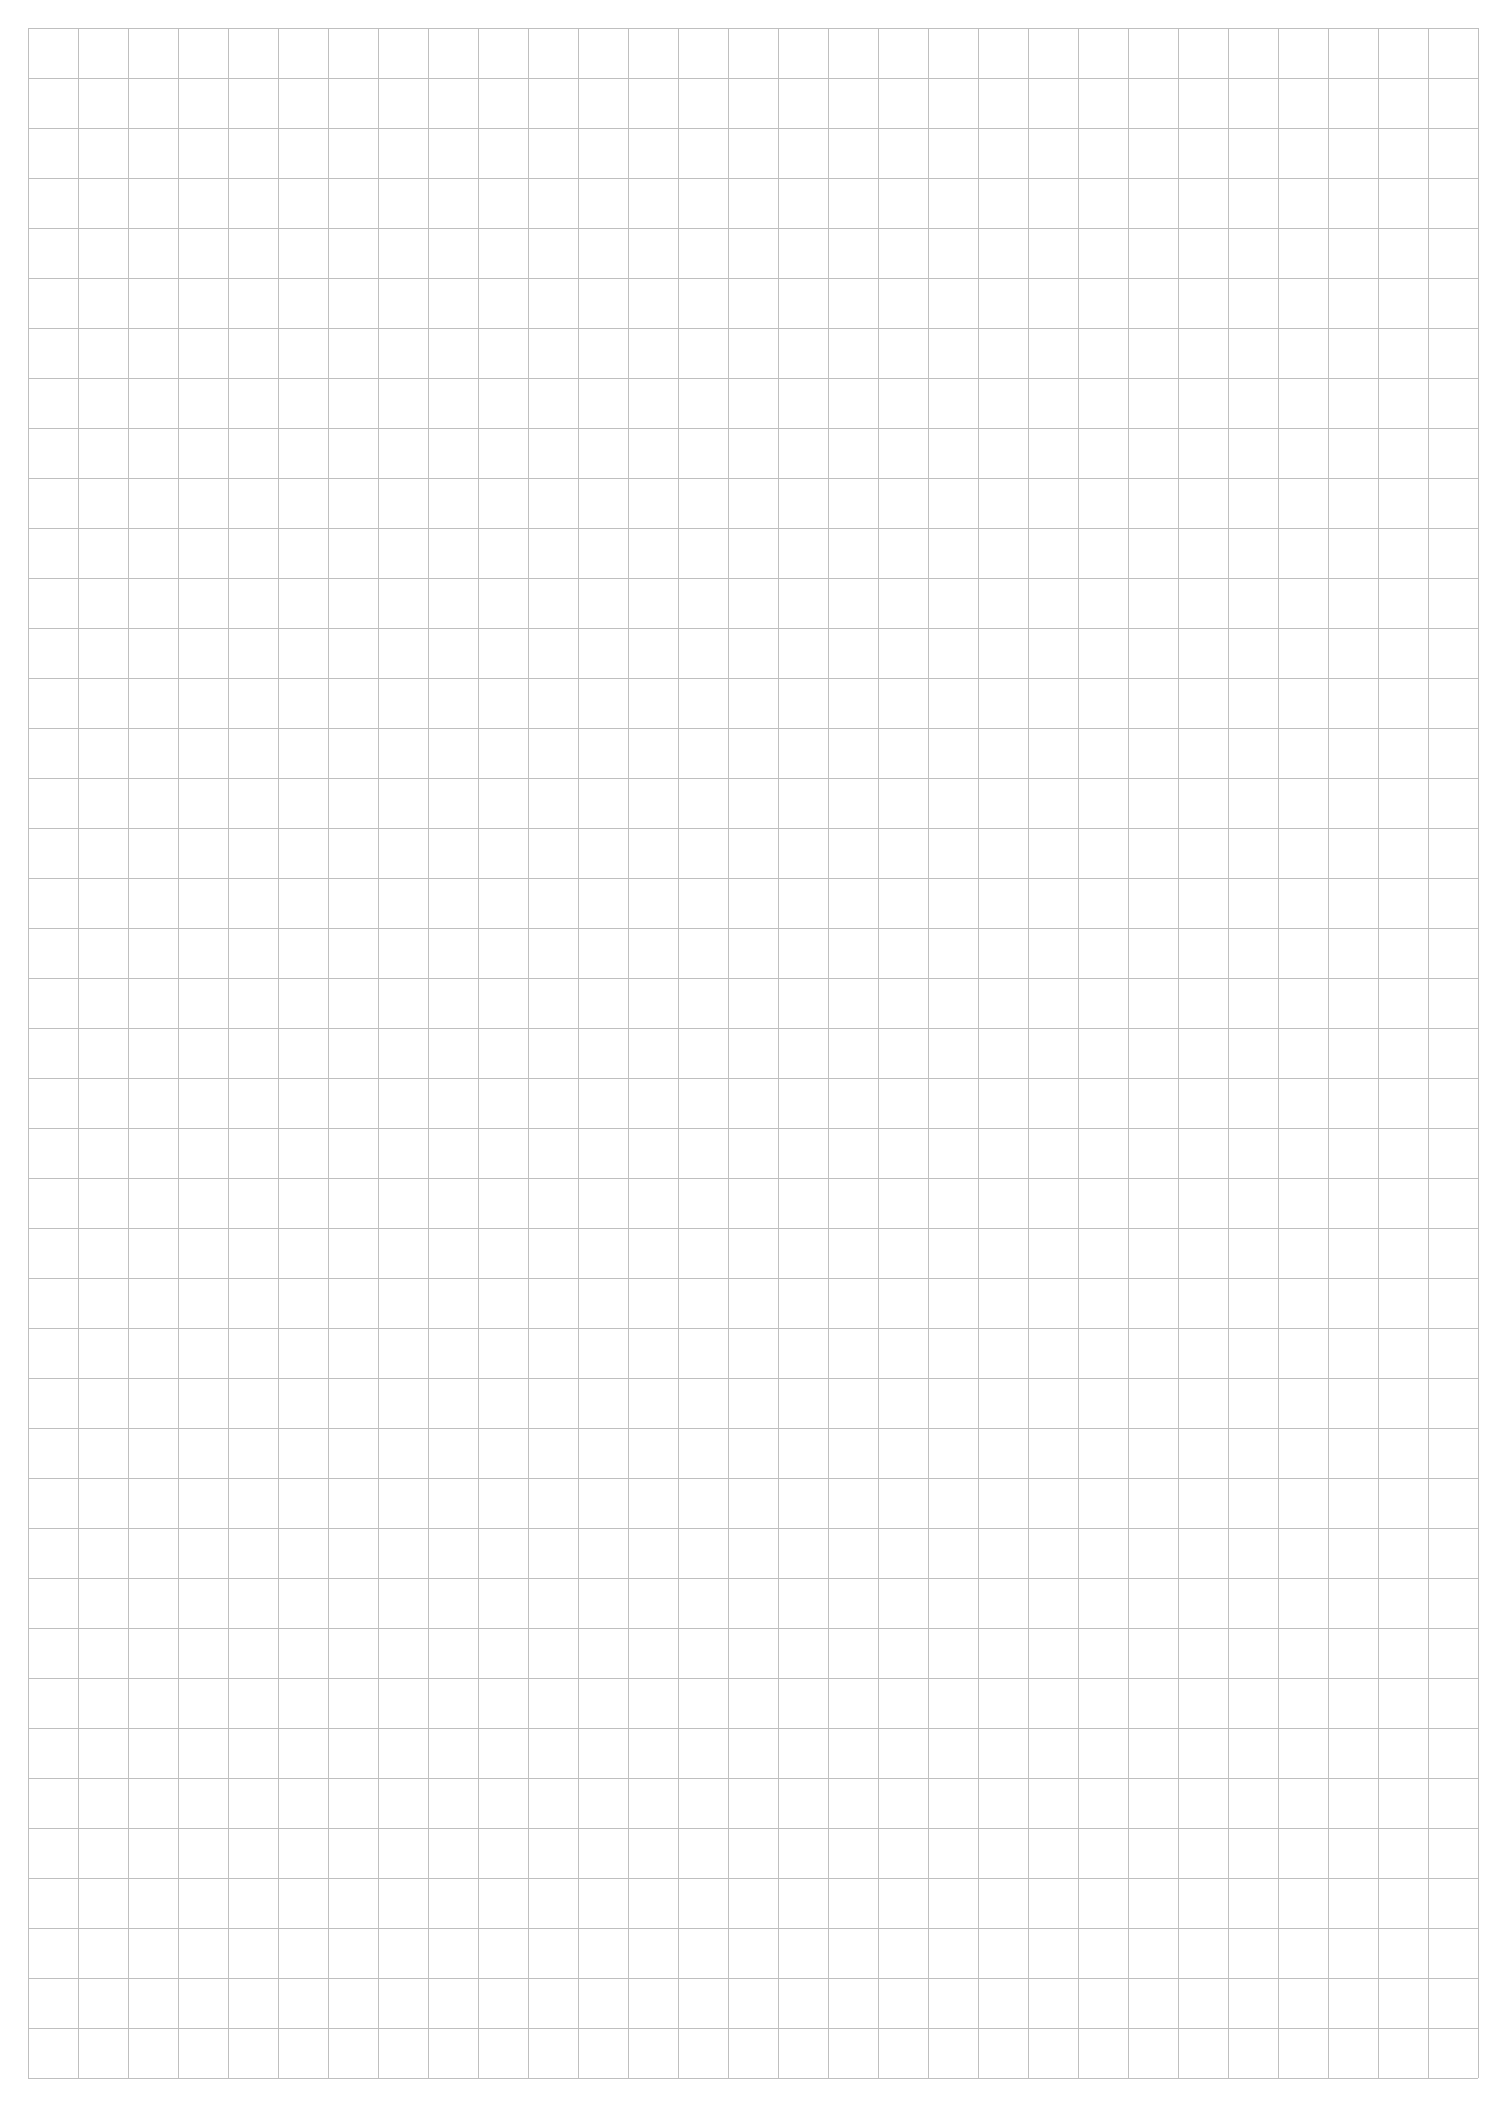
\begin{tikzpicture}[line width=0.1mm]
		\draw[color=gray!50, step=0.25in] (0,0) grid +(7.25in,10.25in);
	\end{tikzpicture}
\end{textblock*}


\begin{textblock*}{7.25in}(1in, 0.375in)
  % \textblockcolor{pink}
	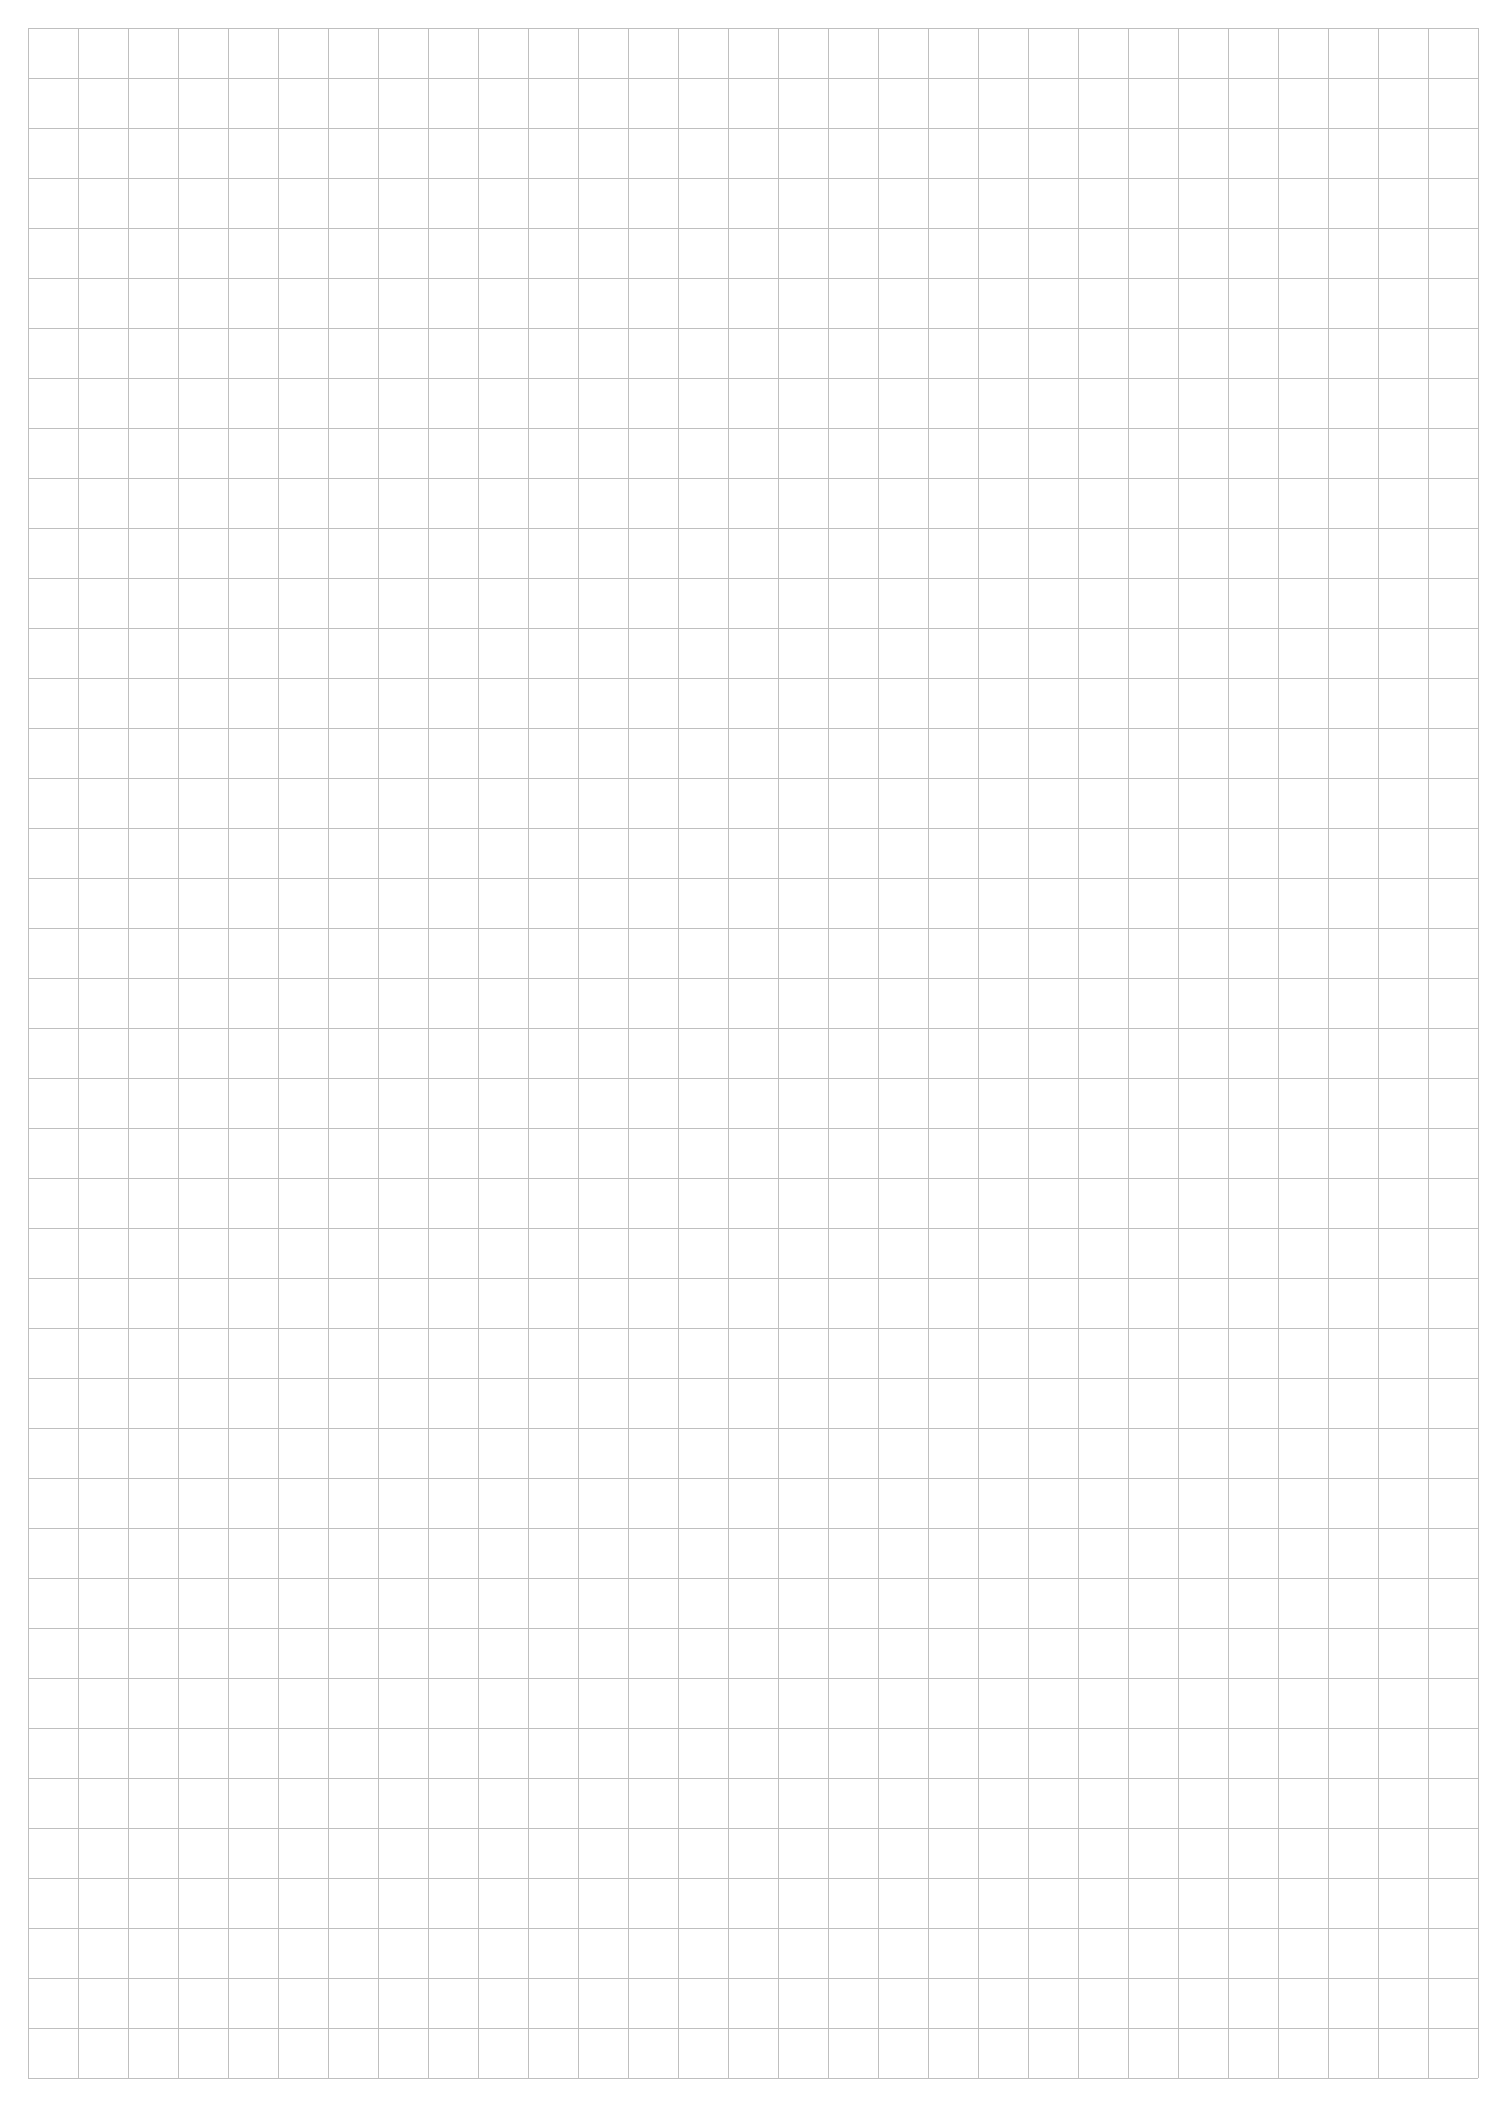
\begin{tikzpicture}[line width=0.1mm]
		\draw[color=gray!50, step=0.25in] (0,0) grid +(7.25in,10.25in);
	\end{tikzpicture}
\end{textblock*}


\begin{textblock*}{6.75in}(1in, 0.225in)
	\cbox{
    \mini[0.4]{
      \vspace{-0.625cm}
      \begin{align*}
        0.36911x + 0.61633y & = 2011.1 \\
        0.78748y - 0.92938x & = 0
      \end{align*}
    }
    \hfill
    \mini[0.4]{
      24) and 25) Find the values of $x$ and  $y$
    }
    \vspace{-0.25cm}
  }  
\end{textblock*}


\begin{textblock*}{6.75in}(1in, 5in)
	\cbox{
    \mini[0.4]{
      \vspace{-0.625cm}
      \begin{align*}
        F_{BC}\sin15^\circ + F_{AC}\cos35^\circ + 1030.1 & = 0 \\
		F_{BC}\cos 15^\circ+F_{AC}\sin35^\circ           & = 0
      \end{align*}
    }
    \hfill
    \mini[0.4]{
      26) and 27) Determine $F_{AC}$ and $F_{BC}$
    }
    \vspace{-0.25cm}
  }  
\end{textblock*}



\end{document}